% ---------------------------------------------------------------------------
% Author guideline and sample document for EG publication using LaTeX2e input
% D.Fellner, v1.13, Jul 31, 2008

\documentclass{egpubl}
\usepackage{eurovis2014}

% --- for  Annual CONFERENCE
% \ConferenceSubmission   % uncomment for Conference submission
% \ConferencePaper        % uncomment for (final) Conference Paper
% \STAR                   % uncomment for STAR contribution
% \Tutorial               % uncomment for Tutorial contribution
% \ShortPresentation      % uncomment for (final) Short Conference Presentation
% \Areas                  % uncomment for Areas contribution
% \MedicalPrize           % uncomment for Medical Prize contribution
% \Education              % uncomment for Education contribution
%
% --- for  CGF Journal
% \JournalSubmission    % uncomment for submission to Computer Graphics Forum
% \JournalPaper         % uncomment for final version of Journal Paper
%
% --- for  CGF Journal: special issue
\SpecialIssueSubmission    % uncomment for submission to Computer Graphics Forum, special issue
% \SpecialIssuePaper         % uncomment for final version of Journal Paper, special issue
%
% --- for  EG Workshop Proceedings
% \WsSubmission    % uncomment for submission to EG Workshop
% \WsPaper         % uncomment for final version of EG Workshop contribution
%
 \electronicVersion % can be used both for the printed and electronic version

% !! *please* don't change anything above
% !! unless you REALLY know what you are doing
% ------------------------------------------------------------------------

% for including postscript figures
% mind: package option 'draft' will replace PS figure by a filname within a frame
\ifpdf \usepackage[pdftex]{graphicx} \pdfcompresslevel=9
\else \usepackage[dvips]{graphicx} \fi

\PrintedOrElectronic

% prepare for electronic version of your document
\usepackage{t1enc,dfadobe}

\usepackage{egweblnk}
\usepackage{cite}
\usepackage{url}
%\usepackage{graphicx}
\usepackage{tikz}
\usepackage{float}
\usepackage{capt-of}


\begin{document}

\title[Storytelling and Visualization: A Survey]%
      {Storytelling and Visualization: A Survey}

% for anonymous conference submission please enter your SUBMISSION ID
% instead of the author's name (and leave the affiliation blank) !!
\author[C.Tong \& R.Roberts \& R.S.Laramee]
       {Chao Tong, Richard Roberts
        and Robert S. Laramee$^{1}$
%        S. Spencer$^2$\thanks{Chairman Siggraph Publications Board}
        \\
% For Computer Graphics Forum: Please use the abbreviation of your first name.
        $^1$Swansea University
  %       $^2$Institut f{\"u}r ComputerGraphik \& Wissensvisualisierung, TU Graz, Austria
%        $^2$ Another Department to illustrate the use in papers from authors
%             with different affiliations
       }

% ------------------------------------------------------------------------
\maketitle
\tableofcontents
\section{Introduction And Motivation}

Throughout history, storytelling has been an effective way of conveying information and knowledge \cite{Lidal2013}. In the field of visualization, storytelling is rapidly evolving into a cutting-edge technique that enhances understanding. Many communities have commented on the importance of storytelling of data visualization \cite{segal}. Storytellers tend to be integrating complex visualizations into their narratives in growing numbers. In this paper, we present a survey of storytelling papers in visualization and present an overview of the common and important elements in storytelling visualization. We also describe the challenges in this field as well as present a novel classification of the literature on storytelling in visualization. The benefit is a concise overview and starting point into this rapidly evolving research trend. 

\subsection{Definition And Storytelling Elements}
Story, from the dictionary, means "a narration of the events in the life of a person or the existence of a thing, or such events as a subject for narration" \cite{story1} or "a series of events that are or might be narrated" \cite{story2}. Storytelling is a popular concept that is used in many fields, such as media \cite{segal}, education \cite{Jack1995} and semiotics \cite{Martin1997}.
Storytelling is a technique to present dynamic relationships between story nodes by interaction.
According to Zipes \cite{Jack1995}, storytelling can involve animation and self-discovery, incorporating models, ethical principles, canons of literature, and social standards. In education, a storyteller can improve and strengthen the literacy of students. Also, the storyteller can engage audiences so they feel a desire to read, write, act, and draw. They learn to express themselves critically and imaginatively with techniques they may learn from the storyteller or teacher.

Martin\cite{Martin1997} states that storytelling can consist of three abstract levels: the narrative level which is more general and more abstract. This is the level of story-structure that underlines all discourse. He describes a story or narrative as presenting events and features movement from one state to another by an act of transformation.

The figurative level is a surface level of meaning and the level that is the most concrete. It relates to individual characters and to specific events unfolding in a given space and time. In other words, figurative elements are in a context that corresponds to the physical world and that can be apprehended by the five senses: vision, hearing, smell, taste and touch.

The deep level which is also knows as the thematic level is the level of the abstract or conceptual. It relates to the inner cognitive world as opposed to the outer physical world of the figurative level. It is the level at which interpretations are articulated the fundamental values in the text are discussed.

\subsection{Challenges in Storytelling And Visualization}
Although storytelling has been developing in other fields for years, in visualization, storytelling is a relatively new subject. It faces many challenges.
 
\begin{enumerate}
\item[$\bullet$] Authorship: Authorship refers to writing or creating a book, article, or document or the creator of a work of art in Oxford English dictionary\cite{authoship2} and origin, especially with reference to an author, creator, producer in dictionary\cite{authoship1}. For our purposes, we will adopt a definition of author described by Rodgers\cite{rodgers2011} " an author is best described as an individual solely responsible for the creation of a unique body of work. 
\item[$\bullet$] Narratives: Narrative structures include events and visualization of characters. Narrative visuals contain the transition between events. It involves " using a tool to visually analyze data, and to generate visualizations via vector graphics or images for presentation" and decide "how to thread the representations into a compelling yet understandable sequence"\cite{hullman2013deeper}.
 
\item[$\bullet$] Visualization of transitions: Transitions are the focus of visualization and include both dynamic and static which are techniques of presenting visualization. Are static transitions or dynamic transitions more effective for storytelling in visualization?

\item[$\bullet$]Memorability: Memorability is an important goal of storytelling. A good visualization technique will draw the viewer's attention and increase a story's memorability \cite{bateman}. Can visualization increase the memorability of data information or knowledge?

\item[$\bullet$] Data enhancement and derivation: Data enhancement and derivation refers to the process of creating a data set from one or more sources such as books or films through enhancement process. How can we perform data acquisition from data sources? And how can we store and represent a story at the data level?

\item[$\bullet$] Interpretation: Data interpretation refers to the process of critiquing and determining the significance of important data and information, such as survey results, experimental findings, observations or narrative reports. Does storytelling and visualization aid with data interpretation?

\end{enumerate}

\begin{table*}[htbp]
\centering
\caption{Storytelling Challenges and descriptive captions} 
\centering 
\begin{tabular}{|c| p{4cm}| p{5cm}|p{4cm}|} 
\hline
 & SciVis & InfoVis & Geo-spatial Vis\\ 
\hline
Authorship & Wohlfart,2006 \cite{wohlfat}\par Wohlfart et al,2007\cite{wohlfart2} \par & Gershon et al,2001\cite{Gershon2}\par Cruz et al,2011 \cite{cruz2011} \par Kuhn et al, 2012\cite{kuhn2012} \par  Lee et al,2013\cite{lee2013} \par & Eccles et al, 2007\cite{eccles2007} \par  Lidal et al,2012 \cite{lidal}  \par Lidal et al,2013\cite{Lidal2013} \par Lundblad et al,2013\cite{lundblad2013} \par\\
\hline 
Narrative & & Viegas et al,2004\cite{viegas2004}\par Akashi et al,2007\cite{akaishi2007narrative} \par Fisher et al,2008\cite{fisher} \par Segel and Heer,2010\cite{segal}\par  Hullman et al,2011\cite{hullman} \par Hullman et al, 2013 \cite{hullman2013} \par Hullman et al,2013 \cite{hullman2013deeper} \par Figueiras,2014 \cite{figueiras} \par Figueiras,2014 \cite{figueiras2014tell}&\\ 
\hline
Static Transitions & & Rebortson,2008\cite{Rebortson} \par  Tanhashi et al,2012\cite{Tanahashi} \par Shixia et al,2013\cite{shixia} & Ferreira et al,2013\cite{ferreira2013} \par \\ 
\hline
Animated Transitions & Akiba et al,2010\cite{Akiba} \par & Bederson and Boltman,1999\cite{bedrson}\par Heer et al \cite{heer2007} \par &\\
\hline
Memorability & &  Bateman et al,2010\cite{bateman} \par & Saket et al,2015 \cite{saket2015} \par\\ 
\hline
interpretation &  Ma et al,2012\cite{sci} \par  &  Kosara and Mackinlay,2013\cite{Kosara} \par & \\
\hline
\end{tabular}
\label{table:classification1} 
\end{table*}


\subsection{Classification of literatures}
The Storytelling literature can be divided into various categories: scientific visualization, information visualization, image processing, narratives, static and dynamic transitions, memorability, data enhancement, interpretation and exploration, analysis versus presentation. Here is a description of these categories :
\begin{enumerate}
\item Scientific Visualization vs Information Visualization: Scientific visualization is seen by a user primarily relates to a physical phenomena occurring in nature, such as flow, volume and surface visualization. While information visualization is more concerned with abstract data with no inherent spatial geometry \cite{spence2007}.
\item Static vs Dynamic: Static visualization requires no action from the user and the encoded data is immediately available. While dynamic visualization refers to those representations that go beyond traditional static which includes animation, interaction and real-time display \cite{spence2007}.
\item Visualization Goals: This includes exploration, analysis and presentation. Exploration refers to navigation and browsing undertaken solely with the aim of forming a mental model of part or all of an information space \cite{spence2007}. Analysis refers to a systematic examination and evaluation of data or information by breaking it into its component parts to uncover their interrelationships. And presentation refers to the selection of encoded data and its layout on a display \cite{spence2007}.
\end{enumerate}
\subsection{Survey scope}
The storytelling visualization papers summarised in this survey include the subjects of scientific visualization, information visualization and visual analytic. Storytelling papers from other fields are not included, such as
\begin{enumerate}
\item[$\bullet$] Virtual reality and augmented reality: For example, Santiago et al \cite{santiago2014mogre} present "Mogre-storytelling" as a solution of interactive storytelling. This tool provides different functionalities for creating and customization of scenarios in 3D, enables the addition of 3D models from Internet and enables the creation of virtual story using multimedia and storytelling elements.
\item[$\bullet$] Education:  For example, Cropper et al \cite{cropper2015scientific} address the extent of how Scientific Storytelling benefits our communication skills in the sciences, and the connections they establish with the information itself and others in their circle of influence.
\item[$\bullet$] Gaming:  For example, Alavesa et al\cite{alavesa2013combining} describe the development of a small scale pervasive game which can take storytelling from camp-fire sites to modern urban environments. 
\item[$\bullet$] Multi-media: For example, Chu et al describe a system to transform any temporal image sequence to a comics-based storytelling visualization \cite{chu2015}. 
\item[$\bullet$] Language processing: For example, Theune et al \cite{theune2006generating} develop a story generation system. It can create story plots automatically based on the actions of intelligent agents living in a virtual story world. The derived plots are converted to natural language, and presented to the user by an embodied agent that makes use of text-to-speech.
\end{enumerate}
\section{Authorship for storytelling and visualization}
Authorship refers to writing or creating a book, article, or document or the creator of a work of art according to The Oxford English dictionary\cite{authoship2} and origin, especially with reference to an author, creator or producer \cite{authoship1}. For our purposes, we will adopt a definition of author described by Rodgers\cite{rodgers2011} "An author is best described as an individual solely responsible for the creation of a unique body of work."  Hullman \cite{hullman2013deeper} et al. state, "Story creation involves sequential processes of context definition, information selection, modality selection, and choosing an order to effectively convey the intended narrative".

\textbf{Title:} \textit{Defining and Experiencing Authorship(s) in the Composition Classroom: Findings from a Qualitative Study of Undergraduate
Writing Students at the City University of New York}
\begin{enumerate}
\item \textit{Definition:} An author is best described as an individual solely responsible for the creation of a unique body of work \cite{rodgers2011}.
\item \textit{The Concept:} Presenting the findings of a qualitative study of undergraduate writers at The City University of New York, Hullman explores student perspectives on models of authorship, the relationships between these models and student experiences of authorship in different writing situations, and proposes the importance of distinguishing between the multiple models and definitions of authorship and the rhetorical contexts associated with each \cite{rodgers2011}.
\item \textit{Case study:}
Rodger develops a qualitative study on 800 students on the definition of authorship and their rhetorical contexts over a one-hour interview.
\begin{enumerate}
\item Students defined authors as "[people] who see writing as being beyond a hobby," and as a term that should be applied only to those
individuals for whom writing is "something he or she has to do," "a career," or "an act that will lead to something being published."
\item What emerged as a key difference between groups was the extent to which each clearly separated the definitions of the terms author and writer. Those students who were comfortable consistently identifying themselves as writers defined the term writer as separate and distinct from the term author, whereas those students who did not clearly separate the two terms, but instead used elements of one definition to inform their definition of the other, were not comfortable consistently identifying themselves as writers.
\end{enumerate}
\end{enumerate}

All papers in this section focus on creating new visualizations for storytelling. Wohlfat and Michael \cite{wohlfat} create new volume visualization story for medical applications. Gershon \cite{Gershon2} and Cruz \cite{cruz2011} present the general storytelling for information visualization. Kuhn \cite{kuhn2012}, Lee \cite{lee2013} and Plowman \cite{plowman1999} all develop unique creator tools for storytelling visualization. 


\subsection{Authorship for  Storytelling and Scientific Visualization}
\textbf{Title:} \textit{Story Telling Aspects in Medical Applications}
\begin{enumerate}
\item \textit{Definition:} Storytelling is a new form of interactive volume visualization presentation \cite{wohlfat}.
\item \textit{The Concept:} This paper explores the usefulness of storytelling in the context of volume visualization. It presents a story telling model and divides the concept of volumetric storytelling into story authoring and storytelling constituents. Then it present a volumetric storytelling prototype application, which is based on the RTVR Java library for interactive volume rendering. See figure \ref{fig:VRVis-Wohlfart-Michael}\cite{wohlfat}.
\item \textit{Theory and application}
\begin{enumerate}
\item Storytelling Model: The storytelling model contains a range of hierarchy levels, in top-down order, which are: story node, story transitions, story action group, story action atoms. The story nodes form the corner marks of the story and store the state of the whole scene. Story nodes are connected by story transitions, each consisting of one or multiple story action groups. Each story action group stores the scene changes relative to its preceding action group (or story node) \cite{wohlfat}.

\item Story Authoring Process: The story authoring process contains two steps: a story recording process and a story editing process. The outcome of this recording process is a raw prototype of a story told through volume visualization. The story editing step this raw story is refined until the final story outline is reached \cite{wohlfat}.
\item Story Telling Process: This process is to present volume visualization following story telling model. And the key feature in this part is interaction, including viewing interaction, representing interaction and data interaction \cite{wohlfat}.
\item Storytelling prototype based on RTVR: This shows an image sequence taken from a sample linear volumetric story visualized with their prototype. The distinct story nodes denoted through (N) refer to the key events in the story, which provide an overview first, then details on specific features in the dataset, and at the end a conclusion made by the story author. The necessary story transitions are represented as orange arrows from one story node to the next and are animated in the prototype application. The story consumer may take over some story parameters (e.g.camera angle) already during playback or at the end of the story to further investigate the dataset \cite{wohlfat}.
\end{enumerate}
\item \textit{Related Work :}  This paper is based on previous work of volume visualization \cite{Amy,robert,Ivan} and interactive visualization \cite{merlin}and combine these concepts together to develop a storytelling model for volume visualization.
\item \textit{In this paper, the following visualization techniques are illustrated :} 
\begin{enumerate}
\item illustrative volume rendering, animation
\item scientific visualization/authorship
\end{enumerate}
\end{enumerate}
\begingroup
\centering
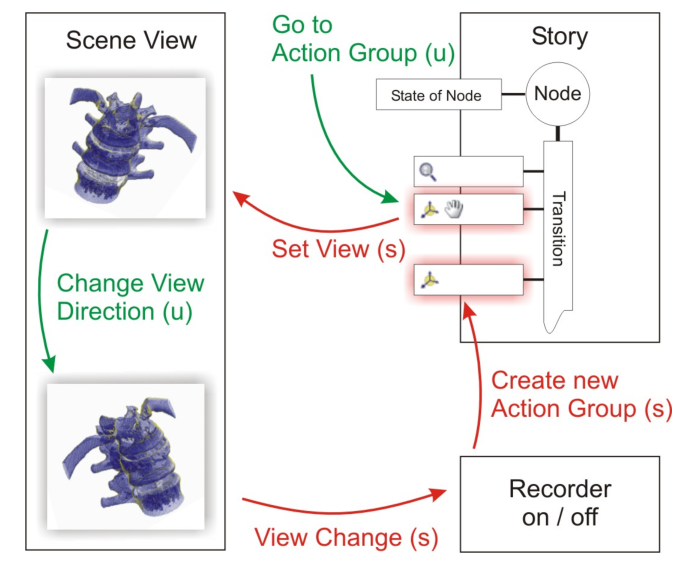
\includegraphics[width=6cm]{./images/VRVis-Wohlfart-Michael}
\captionof{figure}{\textit{The proposed method to author a story is to record the user's natural interaction with the visualisation software. This image shows the process of the story creation. Green annotations represent user interaction and red annotations refer to internal system processes. As soon as the software starts recording, a new story is created and all interactions are logged \cite{wohlfat}.}}\label{fig:VRVis-Wohlfart-Michael}
\endgroup


\textbf{Title:} \textit{Story Telling for Presentation in Volume Visualization}
\begin{enumerate}
\item \textit{Definition:} 
\item \textit{The Concept:} This paper presents a novel approach to volume visualization for presentation purposes that improves the charity
comprehensibility, and credibility of the intended visualization message. Also it combines selected aspects from storytelling as well as from interactive volume visualization to create a guided but at the same time interactive visualization presentation approach, see figure \ref{fig:wohlfart07storyTelling}\cite{wohlfart2}.
\item \textit{Theory and application}
\begin{enumerate}
\item Storytelling Model: the story telling model contains  several hierarchy levels, in top-down order, which are: story node, story transitions, story action group, story action atoms. The story nodes form the corner marks of the story and store the state of the whole scene. Story nodes are connected by story transitions, each consisting of one or multiple story action groups. Each story action group stores the scene changes relative to its preceding action group (or story node) \cite{wohlfart2}.

\item Story Authoring Process: The story authoring process contains two steps: a story recording process and a story editing process. The outcome of this recording process is a raw prototype of a story told through volume visualization. In the story editing step this raw story is refined until the final story outline is reached.\cite{wohlfart2}
\item Story Telling Process: This process is to present volume visualization following story telling model. And the key feature in this part is interaction, including viewing interaction, representing interaction and content interaction.\cite{wohlfart2}
\item CT-dataset visualization story: This story guides the observers through the visualization, puts the contained visual representations
into context to each other and finally introduces them to important features in the data.\cite{wohlfart2}

\end{enumerate}
\item \textit{Related Work:}  This paper is based on previous work of animated visualization \cite{iserhardt} and visual storytelling \cite{tiede} and combines these concepts together.
\item \textit{In this paper, the following visualization techniques are illustrated :} 
\begin{enumerate}
\item illustrative volume rendering, animation
\item Scientific visualization/Authorship
\end{enumerate}
\end{enumerate}

\begingroup
\centering
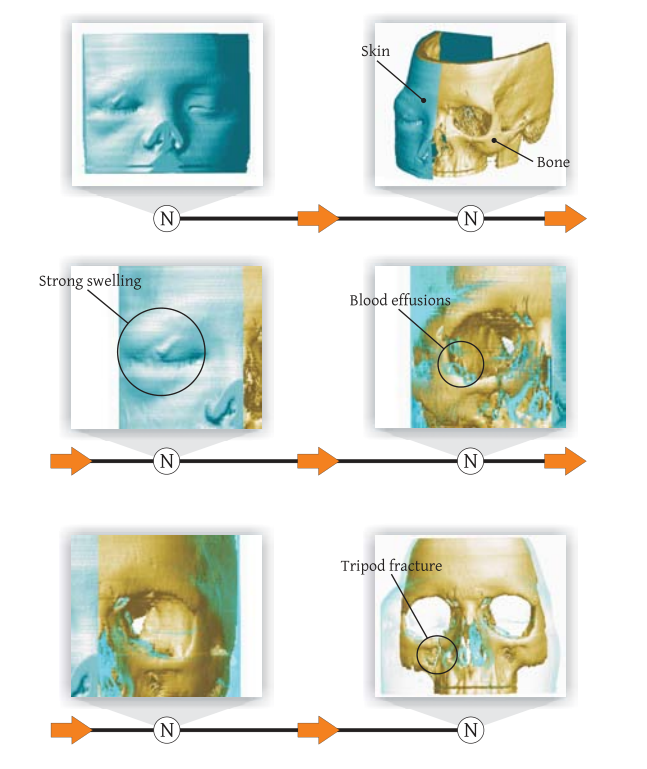
\includegraphics[width=7cm]{./images/wohlfart07storyTelling}
\captionof{figure}{\textit{Here the top two images show an overview of the CT scan data. A partial clipping reveals both the skin layer and bone layer, but shows the full set of data. The middle shows a zoomed view that isolates eye swelling in the image (left), and a filtered view that exposes some blood effusions in the swollen region. The bottom offer a comparison of the non-injured eye with the injured one and shows the cause of the swelling which is attributed to a tripod fracture just below the eye. This design offers the user a macro overview as to lay the foundations of a story background then narrows the scope to view the focal point of the image \cite{wohlfart2}.}}\label{fig:wohlfart07storyTelling}
\endgroup



\subsection{Authorship for Storytelling and Information Visualization}
\textbf{Title:} \textit{What Storytelling Can Do For Information Visualization}
\begin{enumerate}
\item \textit{Definition:} Gershon and Page state that: storytelling enables visualization to reveal information as effectively and intuitively as if the viewer were watching a movie \cite{Gershon2}. 
\item \textit{The Concept:} This paper introduces concept of storytelling and presents advantages of storytelling.
\item  \textit{Examples and Applications:} 
\begin{enumerate}
\item John Thomas of IBM research: By using storytelling, the repeated information of work detail using technology in this research can be deduced into short and memorable information \cite{Thomas}.
\item Enemy positions surround a school: This example presents a situation in which a number of enemy positions surround a school with children trapped inside as de facto hostages as the crossfire fills the space overhead and both sides move toward confrontation \cite{denning}.
\end{enumerate}
\item \textit{Related Work:} This paper is based on previous work of denning \cite{denning} and explain the usage of storytelling in information visualization.
\item \textit{In this paper, the following visualization techniques are illustrated :} 
\begin{enumerate}
\item story board, voice with interaction, bar chart
\item Information visualization/Authorship
\end{enumerate}
\end{enumerate}


\textbf{Title:} \textit{Generative Storytelling for Information Visualization}
\begin{enumerate}
\item \textit{Definition:} Storytelling, in the context of this article, deals with the core of information visualization by extracting relevant knowledge and enhancing its cognition \cite{cruz2011}.
\item \textit{The Concept:} This paper presents generative storytelling as a conceptual framework for information storytelling. It creates stories from data fabulas using computer graphics as a narrative medium. Data fabulas are set of time-ordered events caused or experienced by actors \cite{cruz2011}. 

\item  \textit{System components:} 
\begin{enumerate}
\item Fabulas: Fabulas are set of time-ordered events caused or experienced by actors. Date fabulars and the events, agents, actions, and times represented in a dataset.
\item Generative-storytelling character: Story is formed by characters. It involves the representation of the fabula's actors and the definition of a temporal structure.
\item The conceptual framework: The engine transforming a fabular into story consists two models. The event model creates story timeline and an action model create a set of actors behavior.
\item Applying framework: Visualizing empires decline visualize western empire's decline in the 19th and 20th centuries. See Figure \ref{cruz2011}.
\end{enumerate}
\item \textit{Related Work :} This paper is based on  previous work of narrative theory\cite{naratology1985}, and presents generative storytelling as a conceptual framework for information storytelling \cite{cruz2011}.
\item \textit{In this paper, the following visualization techniques are illustrated :} 
\begin{enumerate}
\item bubble charts
\item information visualization/ authorship
\end{enumerate}
\end{enumerate}


\begingroup
\centering
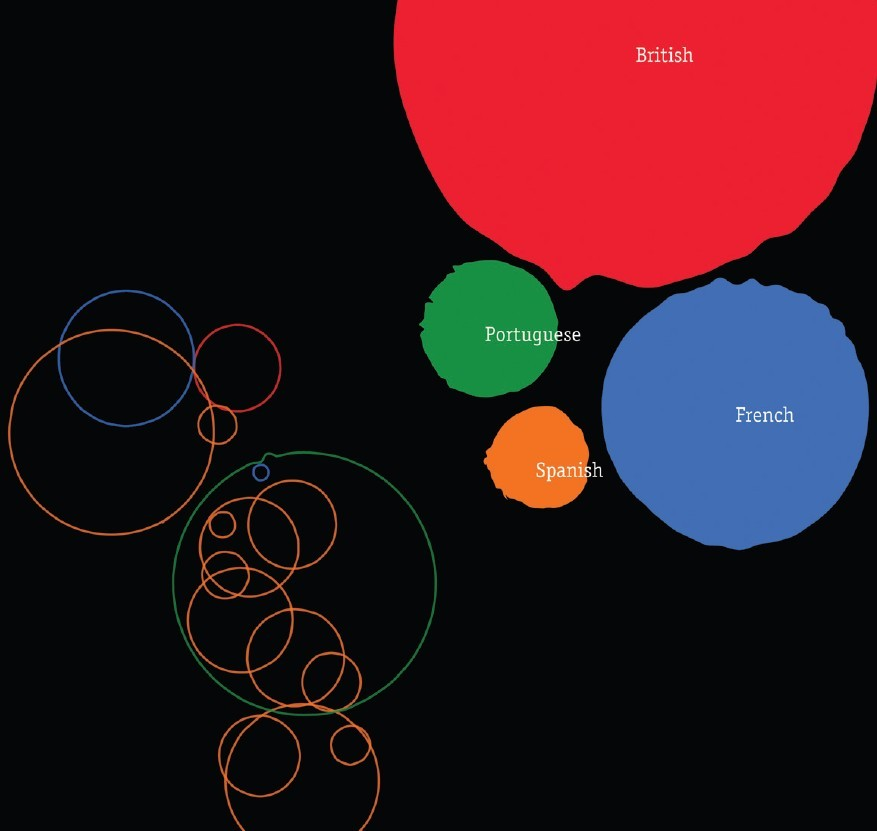
\includegraphics[width=8cm]{./images/cruz2011}
\captionof{figure}{\textit{This figure shows the British hegemony and the newly independent South America in 1891. Each empire and independent territory is a circle whose area is proportional to that entity's land area. Former colonies are unfilled circles with rims in the corresponding empire$’$s color \cite{cruz2011}.}}
\label{cruz2011}
\endgroup

\textbf{Title:} \textit{CodeTimeline: Storytelling with Versioning Data}
\begin{enumerate}
\item \textit{Definition:} 
\item \textit{The Concept:} The CodeTimeline visualisation enables developers who are new to a team to understand the history of the system they are working on.  Designed to show a development team's tribal memory, the software offers a partial replacement for exhaustive documentation, see Figure \ref{fig:kuhn2012} \cite{kuhn2012}.
\item \textit{CodeTimeline Components}
\begin{enumerate}
\item Collaboration View: Collaboration View presents visualizes code ownership and historical patterns in collaboration. 

\item Sourcecloud Flow View: Sourcecloud Flow View presents a word cloud of added and removed vocabulary between software releases. 

\item Lifetime events can be added by users as a frame of reference in each of the visualizations. This method of linking also enables new users to learn more about the history of the developed software. These events can be include anything from email threads to pictures of the team during work.

\end{enumerate}

\item \textit{Related Work:} Ogawa \cite{Ogawa,ogawa2009} presented $"$software evolution storylines$"$ and $"$Code Swarm$"$, which focus on the interactions between developers on projects, but do not focus on telling a story about the software history. Codebook, a concept presented by Begel \cite{begel2010}, outlines a social network that connects software engineers with their shared code base. It encourages interaction with their code and others, enabling a broader understanding of the project they share with other developers.
\item \textit{In this paper, the following visualization techniques are illustrated :} 
\begin{enumerate}
\item Timelines , word clouds
\item Information visualization/authorship
\end{enumerate}
\end{enumerate}

\begingroup
\centering
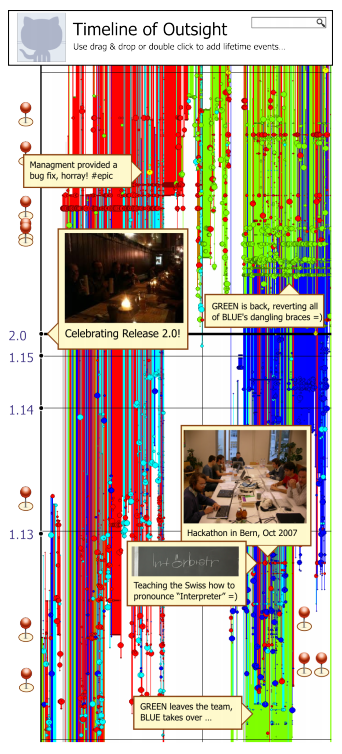
\includegraphics[width=7cm]{./images/kuhn2012}
\captionof{figure}{\textit{This image shows the CodeTimeline collaboration view. Colors denote different user contributions and each line represents the life of files in the code. Sticky notes are added so the users can learn the history of the code beyond the file evolution \cite{kuhn2012}.}}\label{fig:kuhn2012}
\endgroup

\textbf{Title:} \textit{SketchStory: Telling More Engaging Stories with Data through Freeform Sketching}
\begin{enumerate}
\item \textit{Definition:} 

\item \textit{The Concept:} Lee et al. presents SketchStory, a data-enabled digital white board to support real-time storytelling. It enables the presenter to stay focused on a story and interact with charts created during presentation. See Figure \ref{fig:lee2013} \cite{lee2013}.
\item \textit{System design:}
\begin{enumerate}
\item Story preparation: The data-based story is recorded in sketchstory as a sequence of charts in XML files. The charts are linked with specific sketch gestures.
\item Sketchstory Interaction: The presenter draws an example icon then draw sketch gesture for chart invocation. Sketchstory recognizes the gesture and creates the corresponding chart.
\item evaluation: Participating presenters found sketchstory to be good way of storytelling with data, also easy learn and use.
\end{enumerate}
\item \textit{Related Work:}  This paper is based on previous work of storytelling of information visualization \cite{Gershon2,segal} and sketch-based interaction \cite{li2012}, and develops sketchstory system to enhance storytelling in a presentation.
\item \textit{In this paper, the following visualization techniques are illustrated :} 
\begin{enumerate}
\item bar chart, tally chart, line chart, scatter plot, pie chart, map
\item Information visualization/authorship
\end{enumerate}
\end{enumerate}
\begingroup
\centering
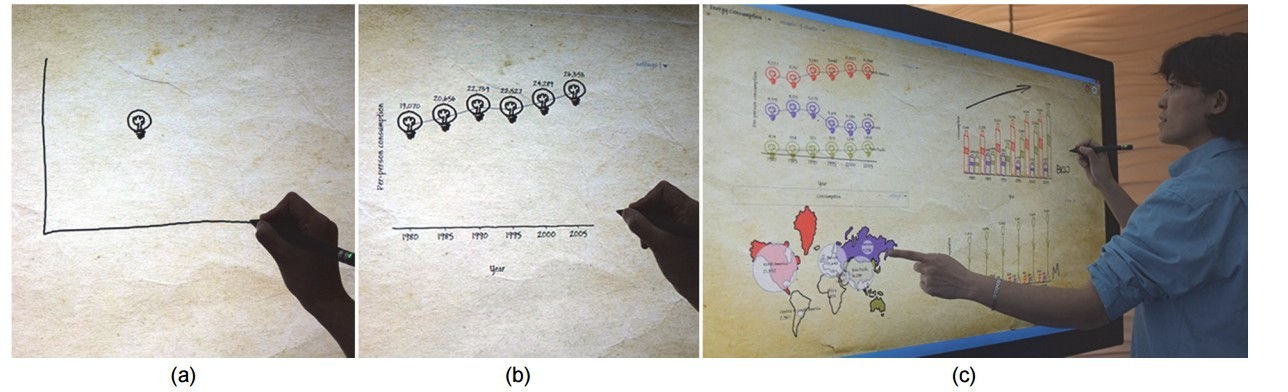
\includegraphics[width=8cm]{./images/lee2013}
\captionof{figure}{\textit{Lee et al show an example of SketchStory in information visualization presentation \cite{lee2013}.}}
\label{fig:lee2013}
\endgroup


\subsection{Authorship for Storytelling and Geo-spatial Visualization}

\textbf{Title:} \textit{Stories in GeoTime}
\begin{enumerate}
\item \textit{Definition:} "Plowman \cite{plowman1999} reports that a narrative specifically refers to the macro-structure of a document in contrast to the term story which refers to both structure and content."
\item \textit{The Concept:} GeoTime events are recorded in X, Y, T, coordinate space. This is used in observation analysis and can make a major contribution to a story telling model. This paper presents the GeoTime stories prototype that combines a geo-spatial map with narrative events to produce a story framework. See Figure \ref{fig:eccles2007} \cite{eccles2007}.
\item \textit{GeoTime Components:}
\begin{enumerate}
\item Annotated Pattern Detection: This system provides functions for simple pattern detection in movement activity. These functions look at possible interactions between people within the narrative, the speed at which they travel, and the type of location that they visit.
\item Narrative text authoring: This enables the analyst to create and present stories found within the data. The story window displays this data as well as discovered patterns. 
\item Story Threading: The system allows multiple stories to connect together if they follow a linear flow. Also simultaneous narratives can be shown in a single image for a direct comparison.
\end{enumerate}
\item \textit{Related Work:}  This system uses a similar approach to Sense.us \cite{heer2007}. Instead of using a blog-type discussion workflow for adding text, Geotime is designed for authoring a single story and annotations are integrated into the data itself.
\item \textit{In this paper, the following visualization techniques are illustrated :} 
\begin{enumerate}
\item GeoTime - event graphs, Geo-spatial visualization, Narrative instance comparison, raw text
\item Geo-spatial/Authorship
\end{enumerate}
\end{enumerate}

\begingroup
\centering
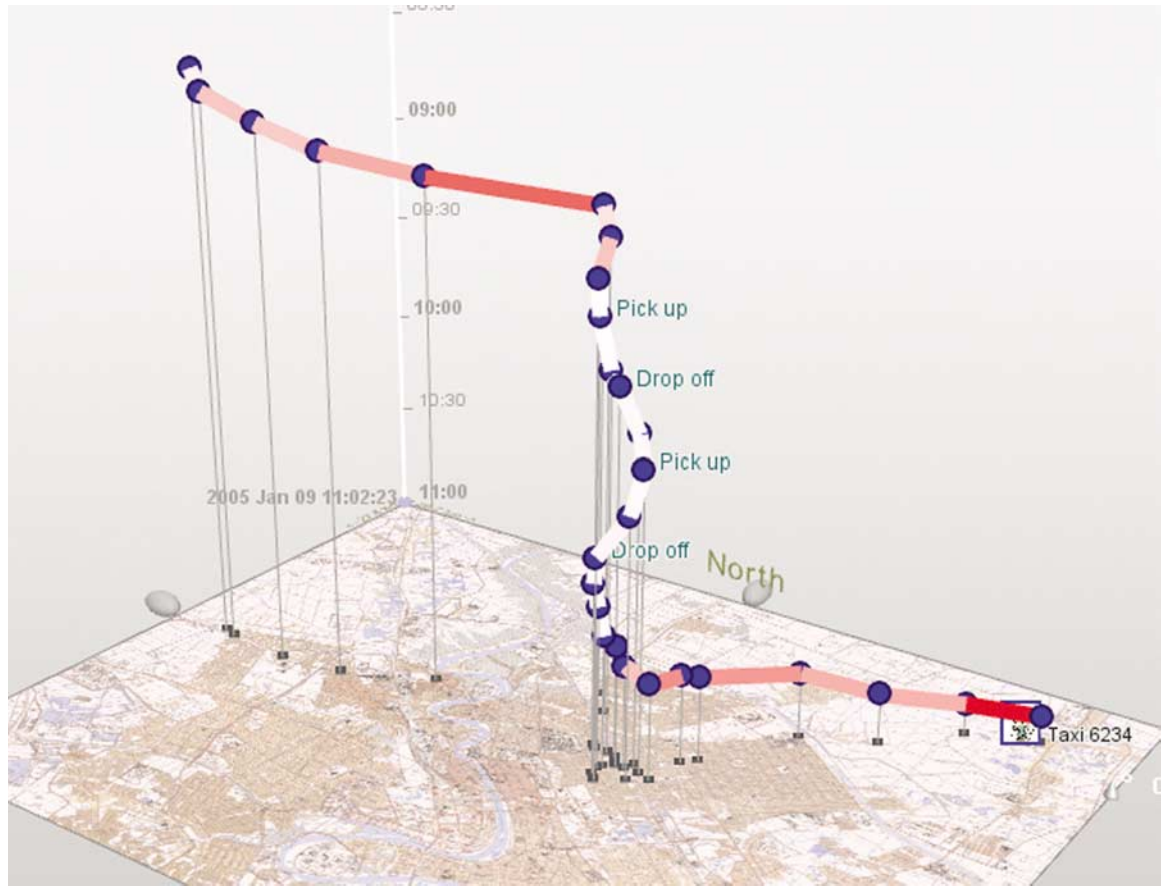
\includegraphics[width=8cm]{./images/eccles2007}
\captionof{figure}{\textit{This shows a GeoTime visualisation instance. The height of the from the base X,Y plain is linked to the temporal dimension. Here you can see a taxi drivers route over the course of a few hours. Each pick up and drop off is labelled and the route is mapped on the X,Y axis using the map \cite{eccles2007}.}}\label{fig:eccles2007}
\endgroup

\vspace{5cm}


\textbf{Title:} \textit{Geological Storytelling:Graphically Exploring and Communicating Geological Sketches} 
\begin{enumerate}
\item \textit{Definition:} Geological Storytelling is a novel graphical approach for capturing and visualizing the reasoning process that leads to a geological model \cite{lidal} \cite{Lidal2013}.
\item \textit{The Concept:} This paper presents a sketch-based interface for rapid modelling and exploration of various geological scenarios. The authors present a concept that handles sketching processed over time and a novel approach for externalizing the mental reasoning process and the process can be presented and evaluated \cite{lidal}\cite{Lidal2013}.
\item \textit{geological storytelling models}:
The geological storytelling models contains three main parts. See figure \ref{fig:Lidal12Geological}.
\begin{enumerate}
\item The Canvas: The canvas is a sketch-based interface where the geologist can draw the geological story on a 2D seismic slice
backdrop, utilizing a pen and paper interaction style.
\item The StoryTree: This is a tree graph representation of all the geological stories, each with its own subtree of story nodes. Individual story nodes can be selected for editing in the canvas. One or more complete story trees can be selected for playback or comparative visualization in the inspect view.

\item The InspectView: This serves two purposes. First, it is a view where a story can be played and evaluated. In addition,
multiple stories can be played synchronized for a side-by-side visual comparison.

\end{enumerate}
\item \textit{Related Work :}  This paper is based on a previous storytelling model \cite{wohlfat} and scientific visualization \cite{sci}, and develops a storytelling model for geological visualization.
\item \textit{In this paper, the following visualization techniques are illustrated :} 
\begin{enumerate}
\item line chart, slicing, geographic information visualization, static graphs
\item Geo-spatial visualization/authorship
\end{enumerate}
\end{enumerate}
\begingroup
\centering
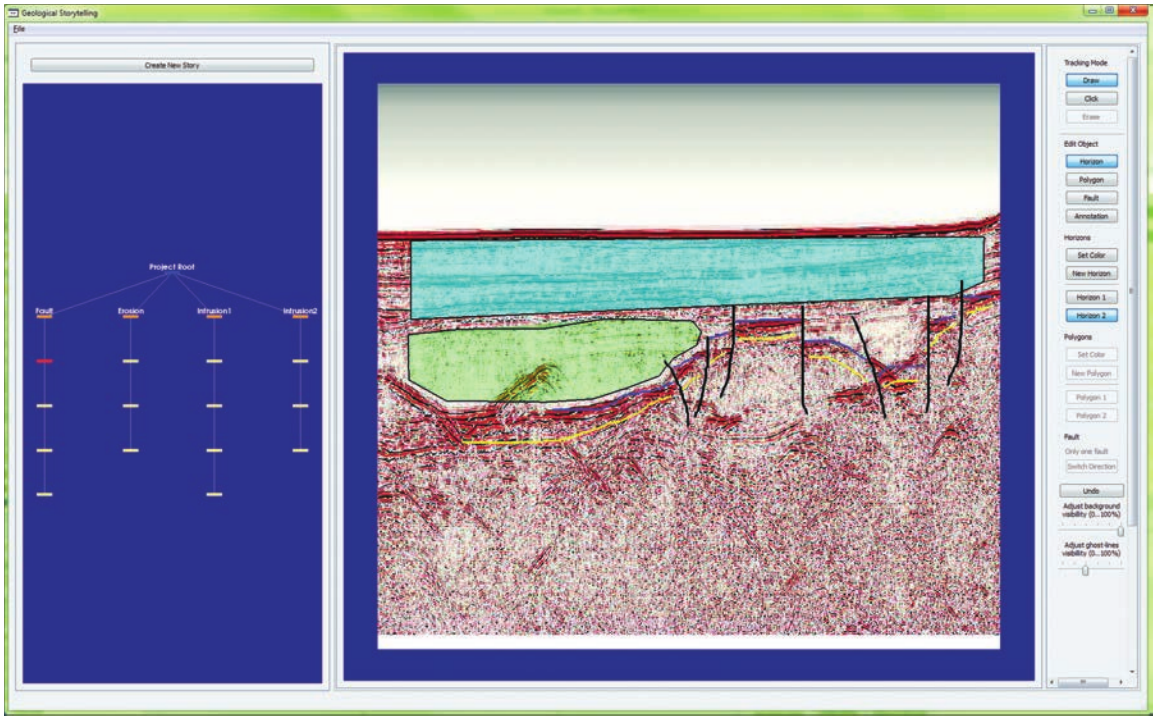
\includegraphics[width=7cm]{./images/Lidal12Geological}
\captionof{figure}{\textit{The sketch-based interface is split into two windows. The Story Tree (left) which shows a tree graph representation of all the geological stories, and The Canvas (right) which shows the sketching interface where the user utilises a pen and paper interaction to record geological sedimentary data. A geological story is built using horizontal lines to separate different geological layers, vertical lines to show fault systems and polygons for highlighting large sedimentary layers. The user can navigate through different geological stories with the story tree and then inspect the geological elements of that story \cite{lidal} \cite{Lidal2013}.}}\label{fig:Lidal12Geological}
\endgroup


\textbf{Title:} \textit{Geovisual Analytics and Storytelling Using HTML5}
\begin{enumerate}
\item \textit{Definition:} Storytelling is one of the most impactful ways to teach, learn, and persuade \cite{lundblad2013}. 
\item \textit{The Concept:} This paper presents Geovisual analytics software with integrated storytelling. It can be applied to large spatial-temporal and multivariate data through dynamic visual user interfaces. 
\item  \textit{Case Study:} 
\begin{enumerate}
\item Multivariate Data Analysis: Using scatter matrix gives the analyst a good overview of all correlations between the selected
indicators. The analyst can here use the scatter matrix as an overview and then steer the scatter plot for interesting detailed combinations over time, See Figure \ref{fig:lun2013}\cite{lundblad2013}.
\item European NUTS2 Regions in Dashboard: The distribution plot presents a special visualization technique that display the variation within individual European countries \cite{lundblad2013}.
\item Motala River Story: The Motala River map is visualized for different story by divided into different layer, such as glyph layer, stream layer, polygon layer and background map layer. It shows the local and total water flow, and water path from source to ocean \cite{lundblad2013}.
\end{enumerate}
\item \textit{Related Work :} This paper is based on the previous work of storytelling concept and work of web-based geovisual tools and integrate storytelling with geovisual analytics software \cite{lundblad2013}.
\item \textit{In this paper, the following visualization techniques are illustrated :} 
\begin{enumerate}
\item interactive visualization, scatter plot, distribution plot, geography information visualization, maps, bar chart
\item Geo-spatial-visualization/authorship
\end{enumerate}
\end{enumerate}

\begingroup
\centering
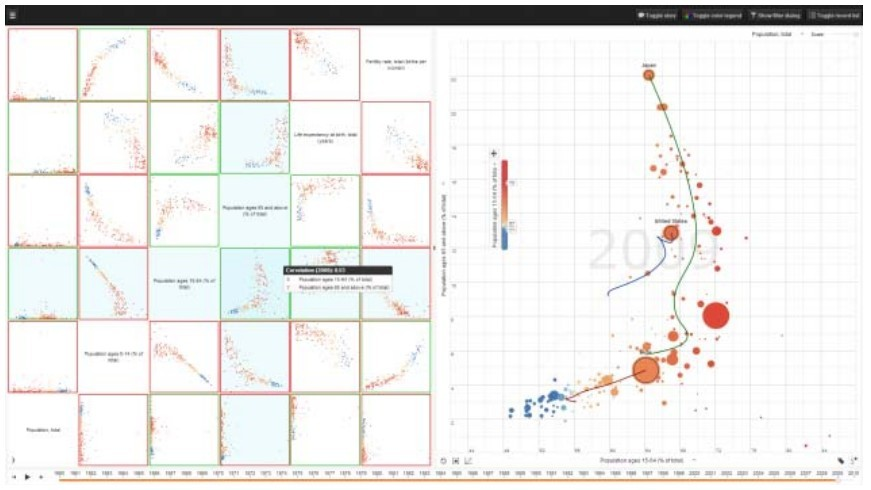
\includegraphics[width=7cm]{./images/lun2013}
\captionof{figure}{\textit{This figure shows  Vislet aimed at a comparative visualization using linked Scatter Matrix and Scatter Plot to analyze national correlation between 6 indicators during 1960-2010 from the World Databank \cite{lundblad2013}.}}
\label{fig:lun2013}
\endgroup


\section{Visualization and storytelling}
Narrative structures include events and visualization of characters. An example narrative can be a simple interface that straightforwardly presents trends in keywords over time \cite{fisher}. Narrative visuals contain the transition between events. It involves "using a tool to visually analyze data, and to generate visualizations via vector graphics or images for presentation" and decide "how to thread the representations into a compelling yet understandable sequence"\cite{hullman2013deeper}. Plowman \cite{plowman1999,eccles2007} reports that a narrative specifically refers to the macro-structure of a document in contrast to the term story which refers to both structure and content. This structuring of evidence, combined with the choice of appropriate rhetorical strategies, is referred to as "the art of storytelling" among literary scholars. Research in narrative visualization points to visualization features that afford storytelling including guided emphasis and structures for reader-driven storytelling. It also includes the principles that govern effective structuring of transitions
between consecutive visualizations in narrative presentations, and how different tactics for sequencing visualizations are combined into global strategies in formats like slideshow presentations.

\textbf{Title:} \textit{Designing Multimedia for Learning: Narrative Guidance and Narrative Construction }
\begin{enumerate}
\item \textit{Definition:} Narrative can be seen as a macro-structure which creates global coherence, contributes to local
coherence and aids recall through its network of causal links and signposting \cite{plowman1999}. 
\item \textit{The Concept:} The focus of Plowman's research is how students make sense of their learning with multimedia by constructing their own narratives in conjunction with the narrative guidance \cite{plowman1999}. The design elements presented by the software constitute
narrative guidance and can be a combination of features specific to interactive media, such as the need for clear navigational procedures, with features associated with traditional media, such as recognizable narrative and a clear relationship between tasks and the macro-narrative. 

\item \textit{Case study}

Plowman has developed three versions of Galapagos as a research tool, based on extended observation of students using commercially available CD-ROMs in schools \cite{plowman1999}.
\begin{enumerate}
\item The linear version is designed in such a way that students are led through the eight sections of the CD-ROM in sequence and it is closest to a traditional narrative as presented in educational television.  The linear version presents a high degree of narrative guidance and little opportunity for learners to decide their own narrative path so they have relatively little control.
\item The resource-based version offers no guidance through the CD-ROM sections and leaves students to define their own route. There is very
little narrative guidance offered and learners have to construct a narrative by making decisions about sequence, so there is a high degree of user control and heavy use of the menu to decide the route. 
\item The guided discovery (GDL) version offers guidance in breaking down the task by providing paths through the material, questions to stimulate enquiries, and direction to specific resources. The GDL version was designed to offer a balance between narrative guidance and support for narrative construction and this is reflected in a more even balance between user and system control. Learners are able to determine sequence and their course of action but are offered guidance in doing so. 

\end{enumerate}
\end{enumerate}

All papers in this section develop methods or structure on how to improve narrative storytelling visualization. Viegas \cite{viegas2004} presents method for improving data memorability. Fisher \cite{fisher} present ways for tracking narrative events over time. Segal and Heer \cite{segal} investigate the design of narrative visualizations and identify techniques for telling stories with data. Hullman \cite{hullman,hullman2013,hullman2013deeper}
design the structure of a visualization to present storytelling.  Figueiras \cite{figueiras,figueiras2014tell} studies how to incorporate narrative elements as storytelling elements.

\subsection{Narrative Information Visualization and Storytelling}

\textbf{Title:} \textit{Digital artifacts for remembering and storytelling: Posthistory and social network fragments}
\begin{enumerate}
\item \textit{Definition:} 
\item \textit{The Concept:} Viegas et al summarize two methods of visualizing email archives with the aim of improving memorability of the data. Both focus on the higher level patterns of the user$'$s email habits. The original goal was for these visualizations to uncover social patterns in the archive, but the resulting visualizations caused the user to be more reflective of the data as opposed to analytic. They look at data points and want to recall the story behind it, even share the visualization with friends. See figure \ref{fig:viegas2004} \cite{viegas2004}.
\item \textit{PostHistory Components}
\begin{enumerate}
\item Visualizes email activity: Two Axis stands for time, and the dyadic relationship between user account holder and each human interaction.
\item Pattern recognition: This includes interaction frequency, interaction rhythm, interaction balance, and archive size.
\item Interface: The visualization includes two main panels; the calendar panel, showing email intensity, and the contacts panel, showing the names of the people being interacted with. 
\item Interaction: When the user clicks on a day square in the calendar panel, the contact panel highlights the names of the people interacted with that day. A name can be clicked on in the contacts panel and each day where that person had corresponded will be highlighted in the calendar panel. The contact panel can be viewed as an animation transitioning through the year of data.
\end{enumerate}
\item \textit{Social Network Fragment Components}
\begin{enumerate}
\item Email header data is used to derive the social context of the communication.
\item Five different relationship types are classified. This can be either directly between correspondents or through mutual recipients in group emails.
\item The Social Network visualization looks at each message and evaluates the role of the user (through the email address used i.e. work, school or personal) and then makes connections regarding the interaction accordingly. 
\item This data is visualized as an animation that evolves over time. Each second represents one day in the archive. A clustered word cloud is used to display the data.
\end{enumerate}
\item \textit{Related Work :} Previous visualizations of online social interaction data have been focused on unraveling the data from the researchers$'$ perspective, whereas these visualizations are for the benefit of the user \cite{boyd2002,donath1995}.
\item \textit{In this paper, the following visualization techniques are illustrated :} 
\begin{enumerate}
\item Clustered word cloud, Animated graph transition
\item information visualization/narrative
\end{enumerate}
\end{enumerate}
\begingroup
\centering
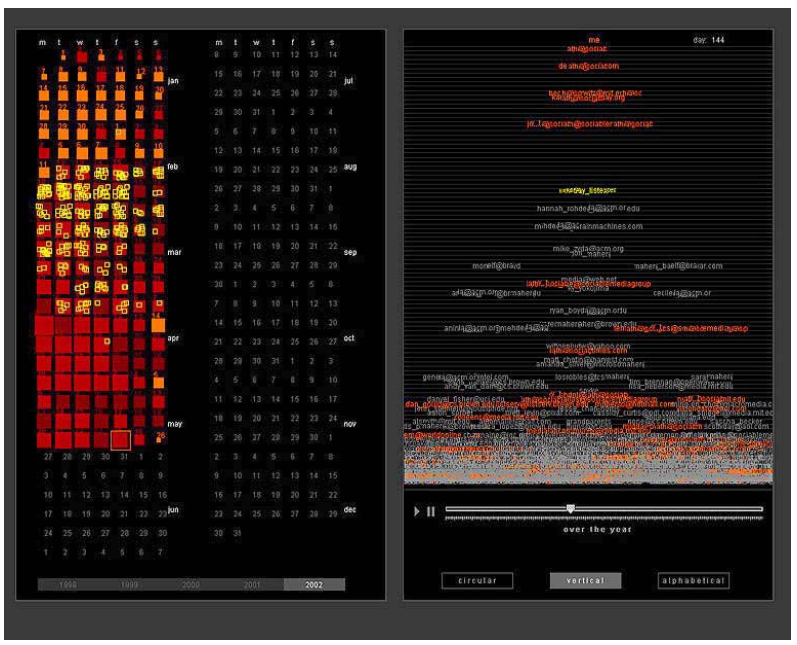
\includegraphics[width=8cm]{./images/viegas2004}
\captionof{figure}{\textit{This image shows the PostHistory visualisation. On the left is the calendar view, showing 365 squares to represent each day of the year (This image only shows data up until May). Size corresponds to the volume of emails sent on that day. The colour highlights a specific recipient that has been selected in the contact panel (left). The contact panel shows all the contacts the user has been corresponding with over the year. A contact can be selected to highlight their interaction in the calendar view \cite{viegas2004}.}}\label{fig:viegas2004}
\endgroup



\textbf{Title:} \textit{Narrative based Topic Visualization for Chronological Data}
\begin{enumerate}
\item \textit{Definition:} Information visualization systems enable users to find patterns, relationships, and structures in data and may help
users gain knowledge or confirm hypotheses \cite{akaishi2007narrative}.  The most basic element in a narrative is a character.
An event occurs through the interaction of a set of characters. A scene consists of a chunk of events. A story consists of a sequence of scenes. A world model is made up of a set of stories.
\item \textit{The Concept:} Akaishi et al propose several methods visualization of chronological data based on the narrative structure of a document \cite{akaishi2007narrative}.
\item \textit{Narrative navigator framework(NANA)}
Akaishi et al. mao each narrative component(world model,story,scene,event,character onto elements of a document, set of stories, sequence of scenes, part of sentence, sets of terms,tern). NANA consists of a decomposition unit and a composition unit. A set of stories is stored in a database by the decomposition unit. In the database, each story is divided into scenes, forming a world model. Appropriate scenes are selected and used by the composition unit to compose a new story. When a user accesses the information, NANA provides the results as a story. The story is presented in various ways. See Figure \ref{akashi}.
\begin{enumerate}
\item Word Colony: The dependency relationship among terms forms a directed graph, called a Word Colony. In a Word Colony, interdependent terms are embedded into the same node. The strength of term dependence is mapped onto the distance between nodes of terms, and term attractiveness is mapped onto the size of node. To visualize this relationship, Akaishi et al use a spring model graph, which is a visual overview of a document.
\item Visualization of topic flows: NANA represents the content of a document as a Topic Sequence and Topic Matrix. Topic Sequence is regarded as
the graphical plot of a document and Topic Matrix represents the relationships among several topic changes. Akaishi et al support users' efforts to find desired parts of documents and to guess the context (plot) of the document.
\end{enumerate}
\item \textit{In this paper, the following visualization techniques are illustrated :} 
\begin{enumerate}
\item Table, Node-link diagrams
\item Information visualization/Narrative
\end{enumerate}
\end{enumerate}

\begingroup
\centering
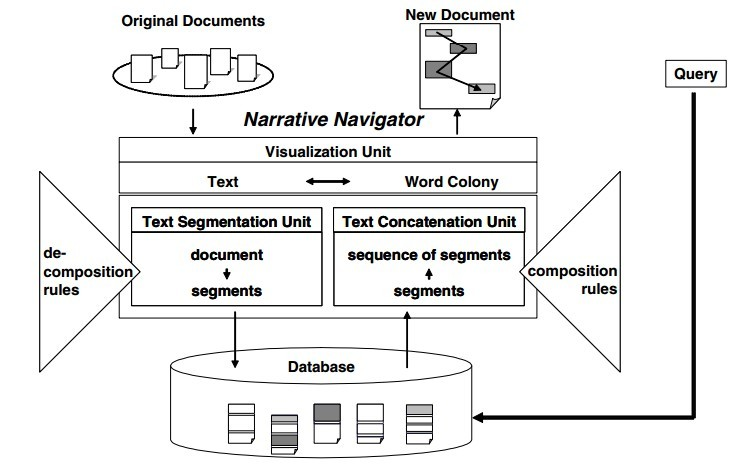
\includegraphics[width=8cm]{./images/akashi}
\captionof{figure}{\textit{This figure shows the structure of Framework of Narrative Navigator \cite{akaishi2007narrative}.}}\label{akashi}
\endgroup


\textbf{Title:} \textit{Narratives: A Visualization to Track Narrative Events as they Develop}
\begin{enumerate}
\item \textit{Definition:} Narrative is a simple interface that straightforwardly presents trends in keywords over time \cite{fisher}.
\item \textit{The Concept:} Fisher et al. present narrative as a way for presenting temporally dynamic data. In this case, narratives help the user by tracking concepts found in news stories change over time. It shows how to piece together complex of information and examine multiple variables, See Figure \ref{fisher} \cite{fisher}.
\item \textit{Case Study:}
\begin{enumerate}
\item Design requirements and scenarios: The first step is based on a business analysis task to find trends and public relations. In this case study, the requirement is to find out how a topic has developed over time and to see the evolution of the latest and most interesting stories \cite{fisher}.
\item System design: This includes data acquisition, temporal visualization, using other tools for correlation, understanding readership, and adding feature in narratives. The narratives project is based on Microsoft's Live Labs which provides real time data acquisition. Temporal visualization enables us see how a small group of words evolves over time relative to one another. By analysing the form of correspondence and understanding readership, additional features can be added into the narrative project \cite{fisher}.
\end{enumerate}
\item \textit{Related Work:} This paper is based on previous work in topic detection and tracking\cite{dubinko2007} \cite{russell2000}, and temporal visualization \cite{van1999}, and presents narrative as a new technique in visualization \cite{fisher}.
\item \textit{In this paper, the following visualization techniques are illustrated :} 
\begin{enumerate}
\item line chart, static graph
\item information visualization/narrative
\end{enumerate}
\end{enumerate}
\begingroup
\centering
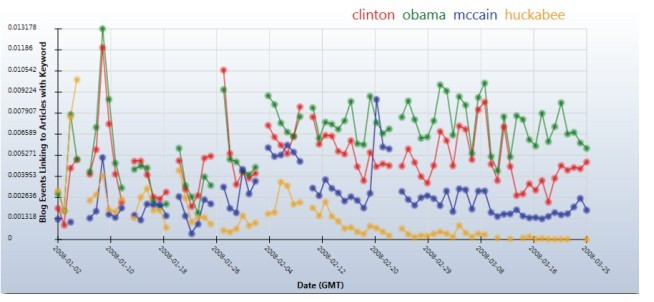
\includegraphics[width=7cm]{./images/fisher}
\captionof{figure}{\textit{This figure shows daily references to four US presidential candidates from January 1 to March 26, 2008. Time
passes along the x axis for each candidate; number of mentions of the term along the y \cite{fisher}.}}
\label{fisher}
\endgroup

\textbf{Title:} \textit{Narrative Visualization: Telling Stories with Data}
\begin{enumerate}
\item \textit{Definition:} Segel and Heer state that storytelling  is revealing stories with data and using visualization to function in place of written story \cite{segal}.The Oxford English Dictionary define narrative as "an account of a series of events, facts, etc., given in order and with the establishing of connections between them". 
\item \textit{The Concept:} This paper investigates the design of narrative visualizations and identifies techniques for telling stories with data graphics and challenges with the salient dimension of visual storytelling. They describe seven genres of narrative visualization: magazine style, annotated chart, partitioned poster, flow chart, comic strip, slide show, and video. See Figure \ref{fig:segelheer} and discusses directions for future reader-centric research \cite{Heer1}.
\item  \textit{Case Studies:} 
\begin{enumerate}
\item New York Times visualization on steroid usage in sports: one larger image and line chart are combined with small images, line charts and bar charts to illustrate the usage of steroids status over 30 years. The visualization incorporates visual highlighting and connecting elements leading viewing order \cite{steroids}. Seasons of player is mapped to the x axis, the amount of steroids is mapped to the y axis, and different colors represent different players.
\item New York Times visualization on budget forecast: a progress bar is used to describe the accuracy of past white house budgets predictions \cite{budget}. The time is mapped to x-axis, and budget situation is mapped to y-axis.
\item Afghanistan nation-building development project: This is a interactive geographic visualization with details on-demand sliders that present the status of Afghanistan nation-building development projects \cite{afghanistan}. Opium cultivation is mapped to the color, and conturies are shown on the map. Time can be changed from 2005 to 2009 by dragging the control bar.
\item Gapminder, Human Development Index: The Gapminder visualization uses animated bubble charts to show possible detrimental effects on a person's ability to follow trends \cite{gapminder2}. Continent is mapped to color, region is mapped to each bubble, and size is mapped to bubble size, position is mapped to average yearly income.
\item Minnesota Employment Explorer: This example shows how mouse-hover provides details-on-demand, double-clicking an industry triggers a drill-down into that sector while an animated transition updates the display to show sub-industry trends \cite{heer2}. Colour represents different industries, the x-axis represents the time, and the y-axis represents employment.
\end{enumerate}
\item \textit{Related Work:} This paper is based on previous work of narrative structure, visual narratives and storytelling with data visualization \cite{Heer1} which observes the storytelling potential of data visualization and drawn parallels to more traditional media. This paper identifies salient design dimensions, clarifies how narrative visualization differs from other storytelling forms and how these differences introduce both opportunities and pitfalls for its narrative potential.
\item \textit{In this paper, the following visualization techniques are illustrated :} 
\begin{enumerate}
\item line charts, bar charts, bubble charts, geographic information visualization 
\item Information visualization/narrative
\end{enumerate}
\end{enumerate}


\begingroup
\centering
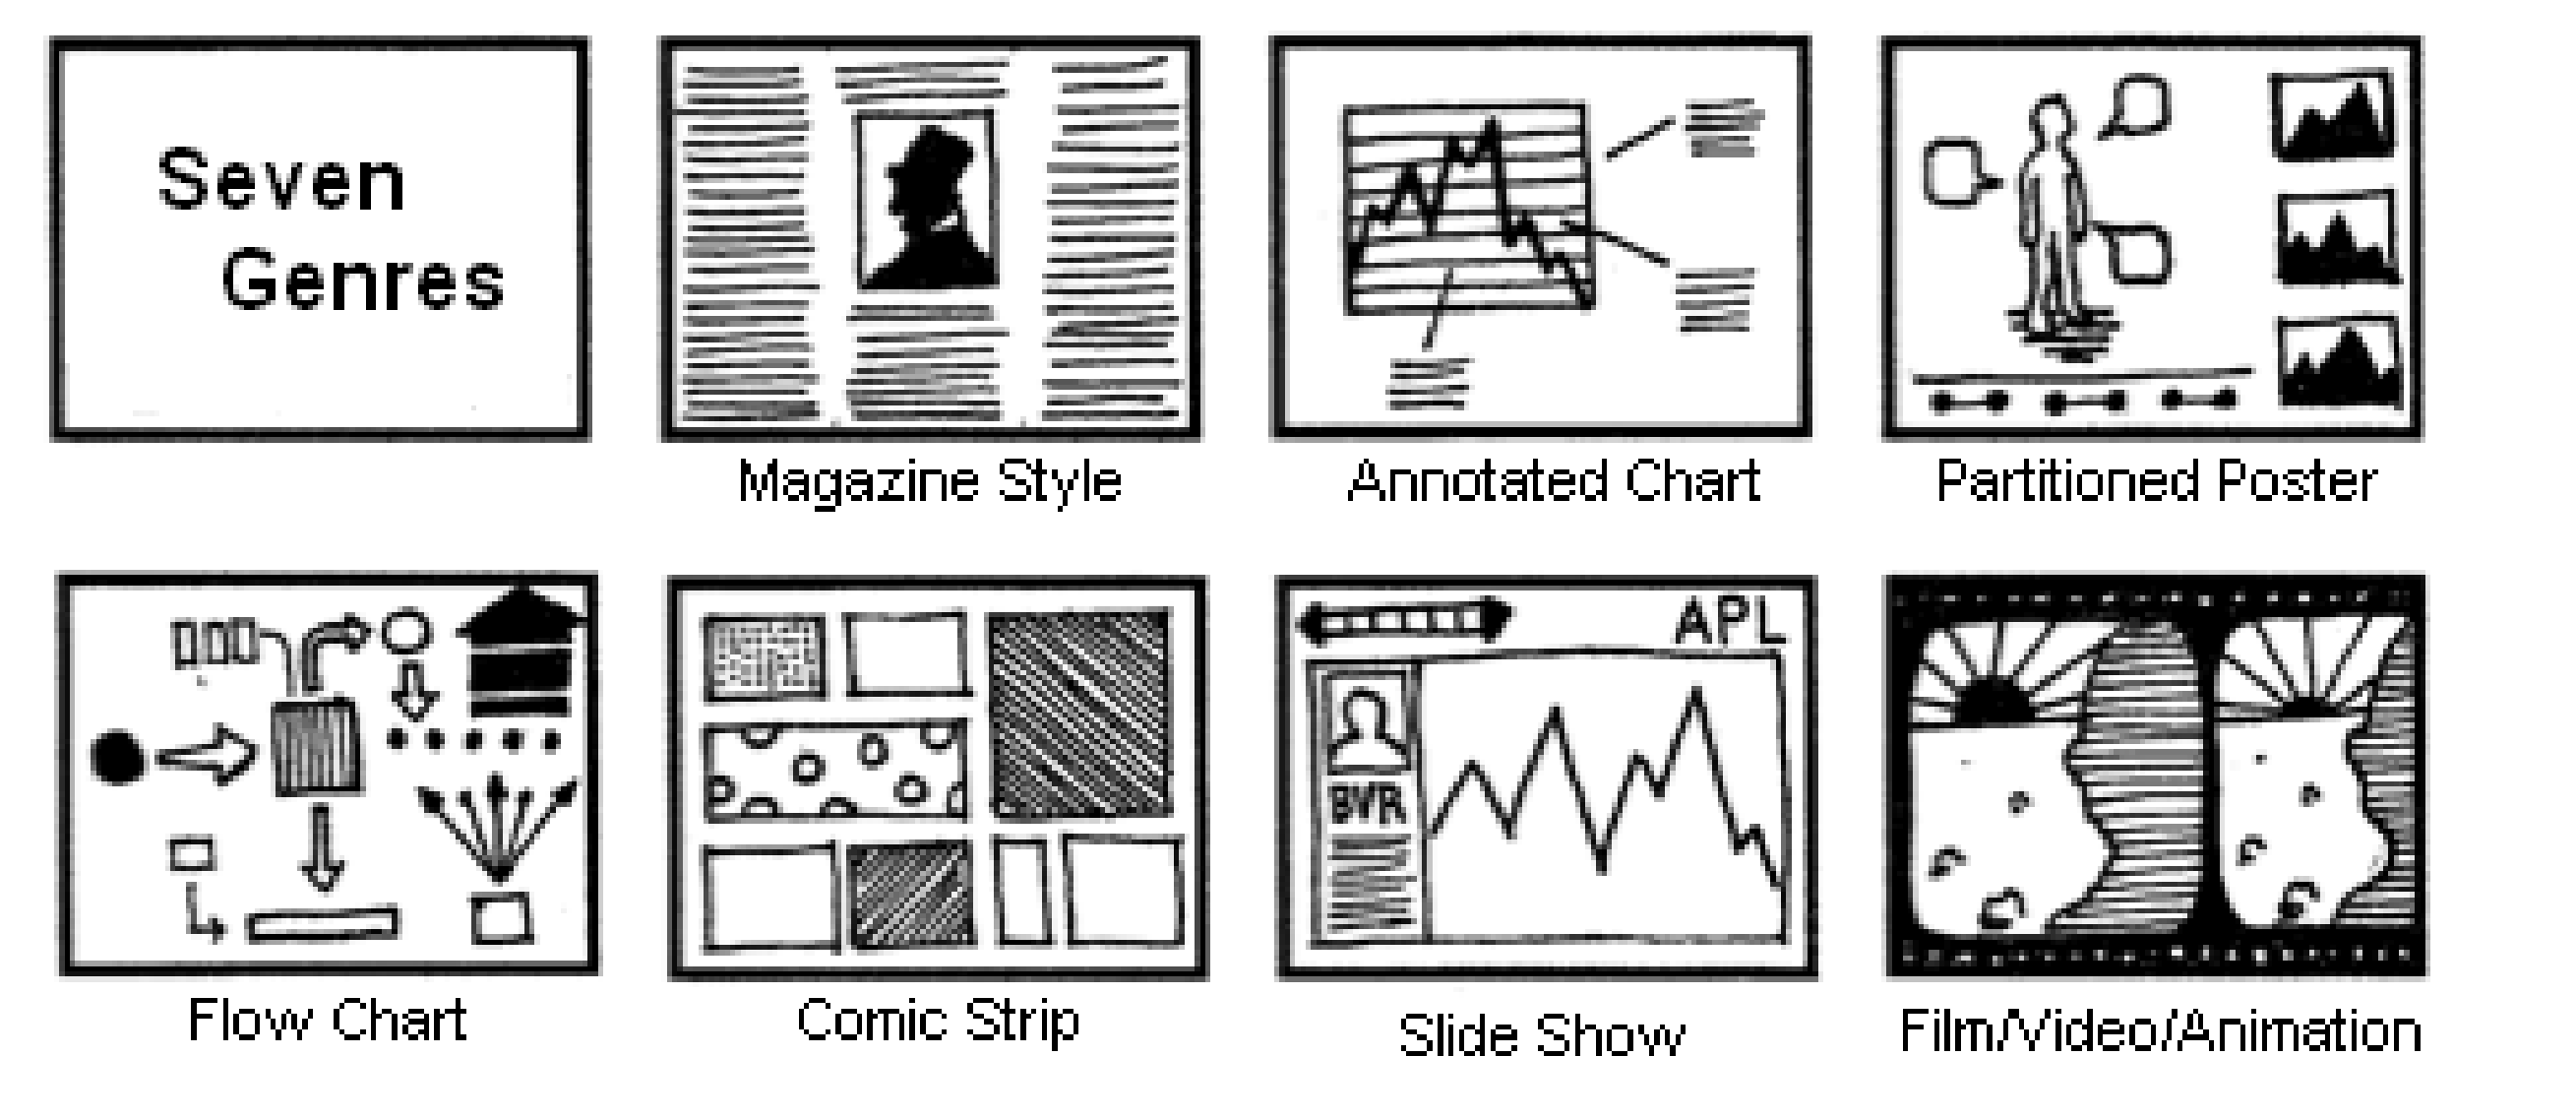
\includegraphics[width=8cm]{./images/segelheer}
\captionof{figure}{\textit{This shows the seven genres of narrative visualization presented by Segal and Heer\cite{segal}. These vary in terms of the number of frames and the ordering of their visual elements. A video, for example has a strict ordering and high frame number, whereas a `Magazine Style' poster may have a few frames in one image that are not strictly ordered. These genre elements dictate if a story is author driven of reader driven. Author driven content uses a linear ordering of scenes and has no interactivity. Reader driven content has no prescribed order to scenes and a high level of interactivity with the reader \cite{segal}.}}
\label{fig:segelheer}
\endgroup



\textbf{Title:} \textit{Visulization Rhetoric: Framing Effects in Narrative Visualization}
\begin{enumerate}
\item \textit{Definition:} Hullman and Diakopoulos state that narrative information visualizations are a style of visualization that often explores the interplay between aspects of both exploratory and communicative visualization \cite{hullman}.
\item \textit{The Concept:} This work contributes to Information visualization  design and theory by providing insight into the types and forms of given rhetorical techniques in narrative visualizations, and the interaction between those techniques and individual and community characteristics of end-users. The author study how rhetorical techniques are used in visualization. They then investigate the resulting effects of these techniques on user interpretation \cite{hullman}.
\item  \textit{Examples and Applications :} 
The authors collect 51 professional narrative visualizations EG from the New York times and bbl. Each visualization is "coded" using theory form semitics, statistics, decision theory, and media and communication studies. The visualizations and categorized according to a selection of rhetorics information access, provenance rhetoric, mapping rhetoric, procedural rhetoric, and linguistic rhetoric. Their work provides a taxonomy of specific information presentation manipulations user in narrative visualization.
\begin{enumerate}
\item Mapping America visualization: The United Stated Census represents a nation-wide attempt to provide an objective view of the demographic of the country. Ethnic group is mapped to color, samples are shown on a map and a single dot represents 200 people \cite{Bloch}.
\item Poll visualization: This visualization summaries the accuracy of political poll predictions from several years and polling agencies in a small multiplies presentation of vertical line graph \cite{McCandless}. Colored bars representing the political parties are drawn to connect data points positioned on the y-axis according to the amount of time prior to the election and on the x-axis according to whether the predictions fell over (to the right) or under (to the left) of a centred vertical line representing complete accuracy (or error of zero). 
\end{enumerate}
\item \textit{Related Work :} This paper is based on previous work of Segel and Heer \cite{Heer1} which make an initial step towards highlighting how varying degrees of authorial intention and user interaction are achieved by general design components in narrative visualization. This work examines the design and end-user interpretation of narrative visualizations in order to deepen understanding of how common design techniques represent rhetorical strategies that make certain interpretations more probable.
\item \textit{In this paper, the following visualization techniques are illustrated :} 
\begin{enumerate}
\item line charts, maps, geographic information visualization,color-coding, bubble charts
\item from data to story
\item information visualization/ narrative
\end{enumerate}
\end{enumerate}

\begingroup
\centering
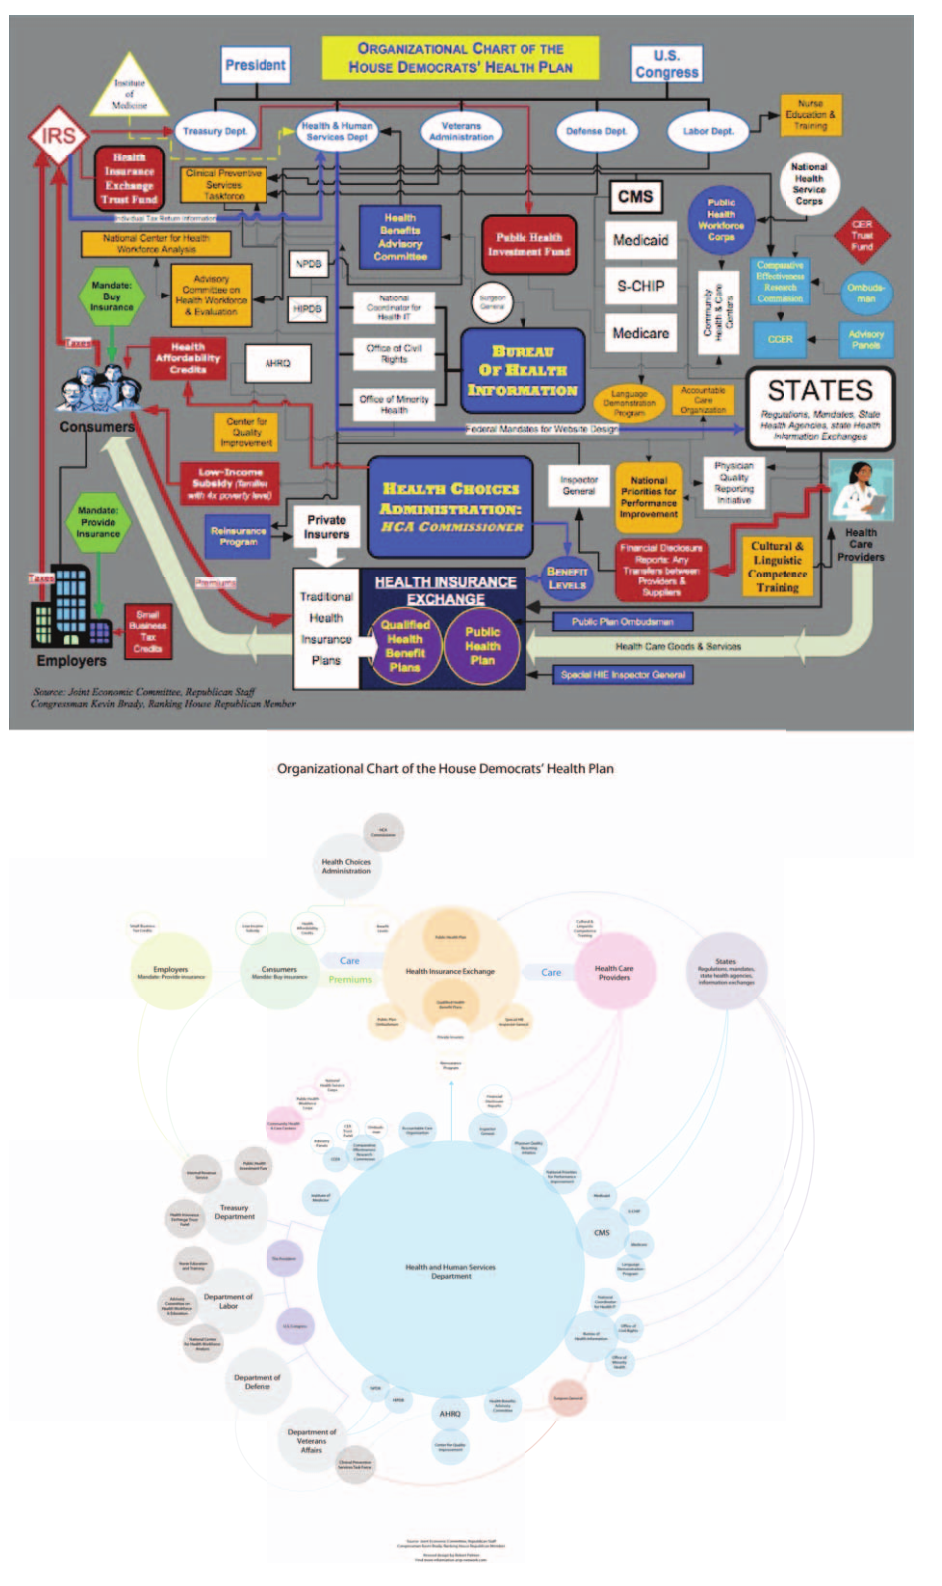
\includegraphics[width=8cm]{./images/vis_rhetoric}
\captionof{figure}{\textit{Figure \ref{fig:vis_rhetoric} shows how data can be window dressed to change the viewers opinion of it. These two images visualise the same data but each illustrator had different intended outcomes. The top image shows an unstructured, complicated graph of conflicting colors and shapes, clearly intended to confuse and obstruct the data, whereas the bottom lays the data out in a simple fashion using consistent shapes and colors \cite{hullman}.}}\label{fig:vis_rhetoric}
\endgroup




\textbf{Title:} \textit{Contextifier: Automatic Generation of Annotated Stock Visualizations}
\begin{enumerate}
\item \textit{Definition:} 
\item \textit{The Concept:} Hullman et al describe a system of contextifier, which automatically produces custom, annotated visualizations from a given article \cite{hullman2013}. 
\item \textit{System overview:}
\begin{enumerate}
\item System architecture: The contextifier contains four main sections: news croups are consist of large set of news articles. A query generator identifies most-relevant company in the article. Annotation selection engine integrates selected feature into annotation. And the graph generator generates line graphs using annotation and series. The flow of information can be seen from figure \ref{fig:hullman2013} \cite{hullman2013}.
\end{enumerate}
\item \textit{Related Work:} This paper is based on previous work in storytelling in visualization \cite{segal} and Kandogan$'$s automatic annotation analytics \cite{kandogan2012}, and developed a system that can automatically generates custom, annotated visualization from a news article of company. Hullman's work places more emphasis on providing background information or perspective on the data than Kandogan$'$s \cite{kandogan2012}
\item \textit{In this paper, the following visualization techniques are illustrated :} 
\begin{enumerate}
\item Time-series graph, line chart, bar chart, histogram,static graph
\item information visualization/narrative
\end{enumerate}
\end{enumerate}

\begingroup
\centering
\includegraphics[width=8cm]{./images/hullman2013}
\captionof{figure}{\textit{This figure shows the architecture of contextifier \cite{hullman2013}.}}\label{fig:hullman2013}
\endgroup


\textbf{Title:} \textit{A Deeper Understanding of Sequence in Narrative Visualization}
\begin{enumerate}
\item \textit{Definition:} 
\item \textit{The Concept:} Hullman et al\cite{hullman2013deeper} outline how automatic sequencing (the order in which to present visualizations) could be approached in designing systems to help non designers navigate structuring decisions in creating narrative visualizations. Their focus is on how linear, slideshow-style presentation can be optimized knowledge of sequencing styles and strategies by incorporation.
\item \textit{Case Study:}
\begin{enumerate}
\item Motivation: Hullman et al. argue that analysts using narrated data presentations could be aided by tools for identifying effective sequences for visualizations.
\item Study Design: They conduct a qualitative analysis of the structural aspects of 42 examples of explicitly-guided professional narrative visualizations. One example is shown in Figure \ref{fig:hullman2013deeper}.
\item Algorithm: They propose a graph-driven approach for finding effective sequences for narrative visualizations informed by their analysis, including defining data attributes for transitions, labelling and maintaining consistency.
\item Evaluation: The result suggests a need for more sophisticated global constraints than simply summing local transition costs to determine the best path through a graph of weighted visualization transitions.
\end{enumerate}
\item \textit{Related Work:} This paper is based on previous work of narrative sequencing\cite{black1979} and narrative visualization\cite{hullman,segal}, and demonstrates that narrative sequencing can be systematically approached in visualization systems.
\item \textit{In this paper, the following visualization techniques are illustrated :} 
\begin{enumerate}
\item bar chart, geo-spatial graph, 
\item information visualization/narrative
\end{enumerate}
\end{enumerate}

\begingroup
\centering
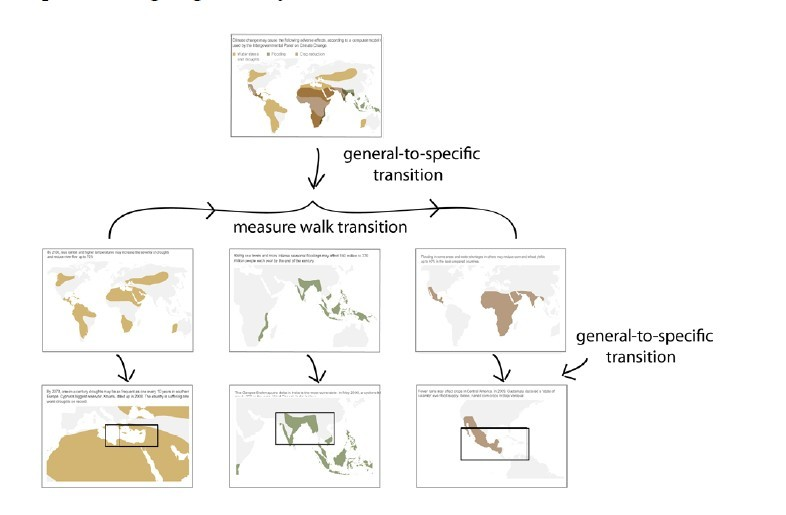
\includegraphics[width=8cm]{./images/hullman2013deeper}
\captionof{figure}{\textit{This figure shows Parallelism in sequencing in the NYT Copenhagen\cite{hullman2013deeper}.}}\label{fig:hullman2013deeper}
\endgroup



\textbf{Title:} \textit{Narrative Visualization: A Case Study of How to Incorporate Narrative Elements in Existing Visualizations}
\begin{enumerate}
\item \textit{Definition:} A visualization with a narrative is set apart from a visualization without through both its structure and its content. A narrative-based visualization attempts to create a natural flow whereby the data has an obvious progression and therefore permits easier understanding and memorability. This area is still evolving research but is found to be very promising \cite{figueiras}.

\item \textit{The Concept:} This paper takes professionally produced visualizations as case studies to analyze how to incorporate narrative elements as storytelling elements. By presenting prototypes of storytelling in selected case studies, Figueiras presents a design study and model for narrative visualization by using storytelling techniques \cite{figueiras}.
\item \textit{Case Study:}
\begin{enumerate}
\item How many households are like yours?: In this figure, users can choose the primary residents and secondary members of a household, then get the number and percentage households. Figueiras \cite{figueiras} introduces short stories describing different kinds of families instead of having only one article about types of families. And this technique engages the user with a focus on creating empathy.
\item What does China censor online?: The figure is a simple tag cloud that only has a title and text shaped on a map of China. Figueiras \cite{figueiras} introduce small tooltips pop up when a user clicks on one region, which provides more detailed information. See figure \ref{fig:figueiras14narrative}. Tooltips provide additional context in the form of tooltips which help explain the possible reasons for censorship. 
\item Death Penalty Statics, Country by Country: This figure is a static visualization with different size of bubbles representing the number of death sentence rulings. Figueiras \cite{figueiras} designs an interaction such that when a user chooses a year, a graph displays the number of death sentences handed out that year, which provides extra temporal information and a redesign into a story. 
\end{enumerate}
\item  \textit{Narrative Strategies:} 
\begin{enumerate}
		
	\item Context: Providing context to a visualization enables the user to make sense of the data using additional information. Without a sufficient amount of context, less meaning can be derived from the data, whereas the addition of context gives the user more information to explore the data and begin to understand features found within it. This is made easier by the development of interactive visualizations and the ability for users to choose what layers of information they see. 
		
	\item Empathy: Although not often associated with information visualization, it has been found that emotive/empathetic visualizations are more memorable and more enjoyable for the user \cite{Kosara}.
		
	\item Time Narrative: Utilizing the temporal nature of data in visualization allows users to mentally map the data by adding a sense of story flow. This improves user memorability and aids in the understanding of the data \cite{Kosara}.
		
\end{enumerate}
\item \textit{Related Work :}  This paper is based on previous work of storytelling \cite{hullman}\cite{sci}\cite{segal} and narrative visualization \cite{fisher}, and develops a model to add storytelling in narrative visualization \cite{figueiras}.
\item \textit{In this paper, the following visualization techniques are illustrated :} 
\begin{enumerate}
\item Interactive graph, text visualization, bar chart, geo-spatial visualization
\item Information visualization/narrative
\end{enumerate}
\end{enumerate}


\begingroup
\centering
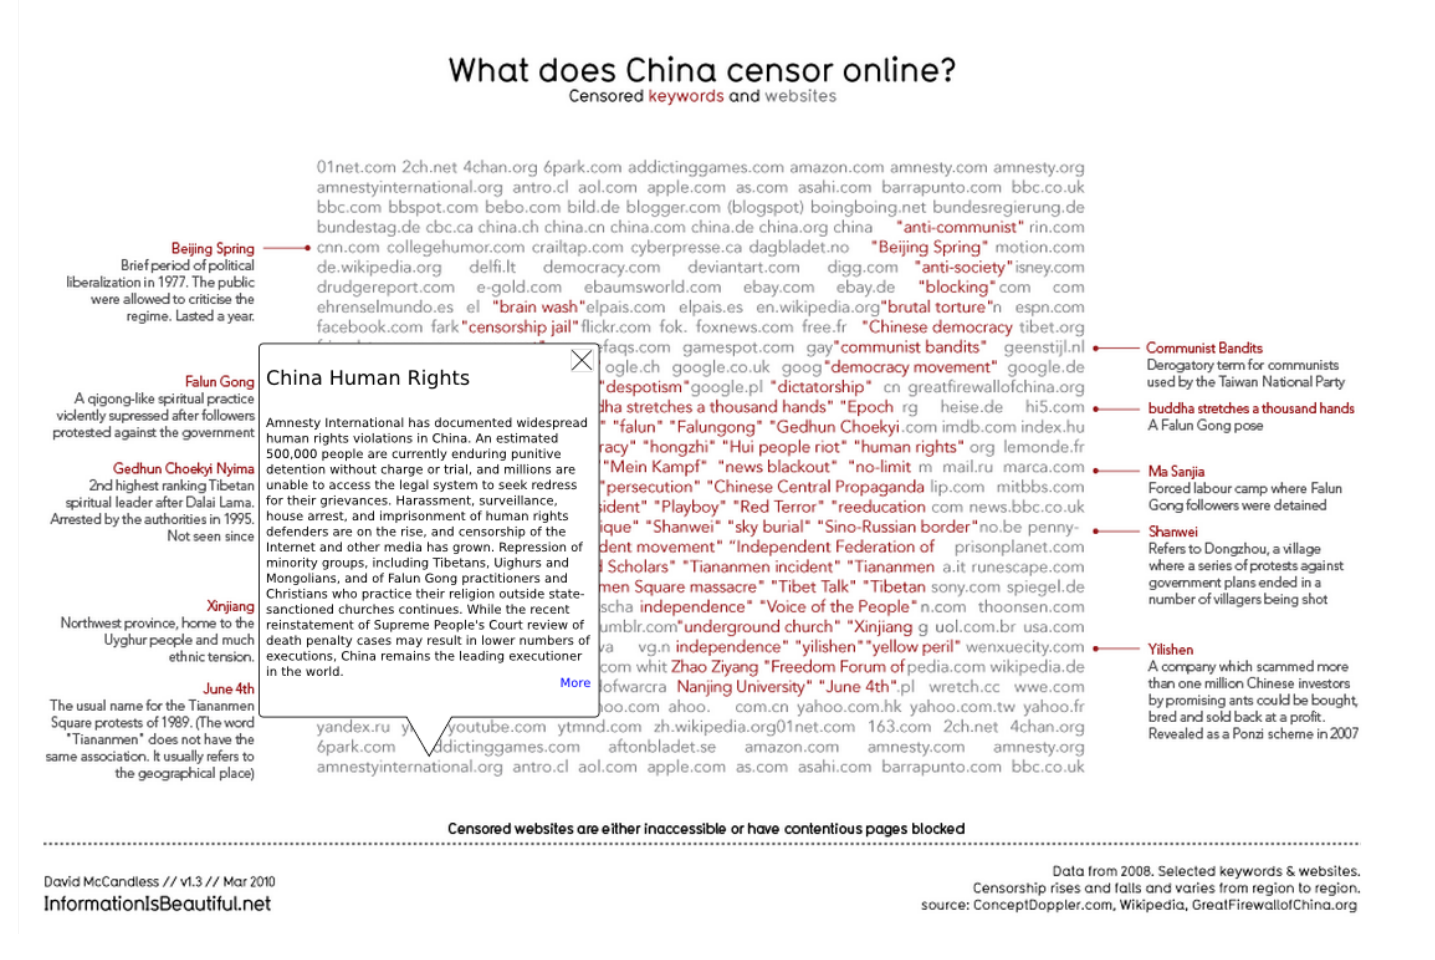
\includegraphics[width=7cm]{./images/figueiras14narrative}
\captionof{figure}{\textit{This is visualization of Chinese online sensorship enhanced with storytelling. An interactive feature is added so that the user can click on an instance of sensorship to learn more about it. This supplies context to the user and also may draw towards an empathetic response from the user \cite{figueiras}.}}
\label{fig:figueiras14narrative}
\endgroup


\textbf{Title:} \textit{How to Tell Stories Using Visualization}
\begin{enumerate}
\item \textit{Definition:} Storytelling aims to simplify concepts, create emotional connection, and provides capacity to help retain information \cite{figueiras2014tell}.
\item \textit{The Concept:} Figueiras presents the results of a focus group study on collecting information on narrative elements. They then suggest strategies for storytelling in visualization \cite{figueiras2014tell}.
\item  \textit{Case Study:} 
\begin{enumerate}
\item Sixteen participants are asked to study 11 information visualizations of different types and different characteristics (Interactive, non-interactive, introductory text, accompanying article, and audio narration). Then they were asked to rate visualizations in terms of  comprehension, navigation, and likability, See Figure \ref{fig:fig2014}. 
\item The participants give high scores to all visualizations, particularly to interactive visualizations. The story suggests that a good storytelling visualization is well-structured and interactive with audience preferences. The results of the user story suggest that interactivity, drilling-down, context, and a sense of relatability and important for users to fell engaged.
\end{enumerate}
\item \textit{Related Work:} This paper is based on previous work of narrative visualization \cite{segal}, and storytelling visualization \cite{Kosara,sci}. The author uses a focus group to examine in storytelling effects in information visualization and storytelling visualization.
\item \textit{In this paper, the following visualization techniques are illustrated :} 
\begin{enumerate}
\item Map, Poster, Photography, Tag Cloud, Drawing, Chart/Diagram, Model
\item Information visualization/Narrative
\end{enumerate}
\end{enumerate}

\begingroup
\centering
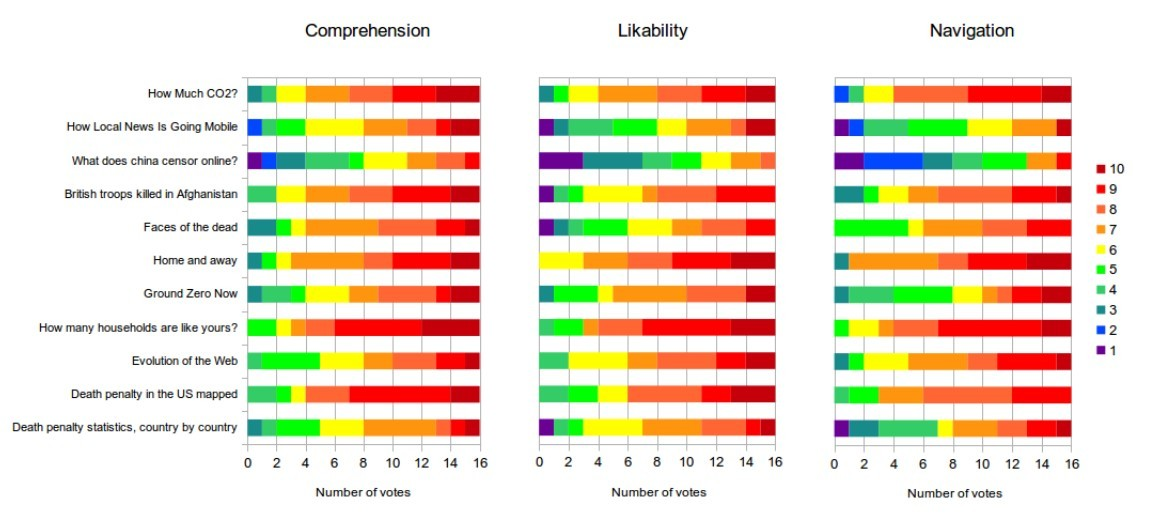
\includegraphics[width=8cm]{./images/fig2014}
\captionof{figure}{\textit{This shows the scores given by participants to each visualization in term of comprehension, likability, and navigation \cite{figueiras2014tell}.}}
\label{fig:fig2014}
\endgroup



\section{Static Transition}
A transition refers to the process or a period of changing from one state or condition to another according to The Oxford English Dictionary \cite{transition}. In visualization, transitions may be the focus of visualization and include both dynamic and static which are alternatives of presenting visualization. Static visualizations are those that do not change with time. 

In this section, the visualization of transitions is generally static. The authors focus on presenting the trend of data along timelines. Roberson \cite{Rebortson} evaluates three approaches of using bubble charts and try to find out which one work best for presentation and analysis. Tanahashi and Ma \cite{Tanahashi} presents a storyline visualization which consists of a series of lines, from left to right along the time-axis.  Liu et al \cite{shixia} design a storyline visualization system, StoryFlow, to generate an aesthetically pleasing and legible storyline visualization. Ferreira \cite{ferreira2013} proposes a method of visualizing a large amount of taxi data consisting of both spatial and temporal dimensions.


\subsection{Information Visualization}
\textbf{Title:} \textit{Effectiveness of Animation in Trend Visualization}
\begin{enumerate}
\item \textit{Definition:} Robertson et al define a trend in data as an observed general tendency. The most common way to see a trend in data is to plot a variable's change over time on a line chart or bar chart. If there is a general increase or decrease over time, this is perceived as a trend up or down \cite{Rebortson}.
\item \textit{The Concept:} This paper proposes two alternatives to animated bubble charts for visualizing trends in multiple dimensions and describes a user study that evaluates the three approaches for both presentation and analysis. In conclusion, it states that traces and small multiples work best for analysis \cite{Rebortson}.
\item  \textit{Examples and Applications:} 
\begin{enumerate}
\item Multi-dimensional trends: The gapminder trendalyzer uses a bubble chart to show five dimensions of data, life expency is mapped to the x axis, infant mortality is mapped to the y axis, population is mapped to bubble size and continent is mapped to color \cite{ted1}.
\item Alternative multi-dimensional trend visualization: A trace visualization provides the user with the ability to select particular bubbles such that the animation shows a trace line for the selected bubble as it progresses  see figure \ref{fig:Robertson} \cite{ted2}.
\item Small multiples visualization: countries can be clustered based on position, size and location. They are further grouped by continent and ordered alphabetically within each group \cite{Tufte}.
\end{enumerate}
\item \textit{Related Work:} This paper based on earlier work by Tversky et al. \cite{tversky} and Baudisch et al. \cite{baudisch}. Previous work is limited to small data set sizes (200 samples or less). Previous work focuses on presentation rather than analysis and relies on animation to show trends over time.
\item \textit{In this paper, the following visualization techniques are illustrated :} 
\begin{enumerate}
\item line charts, bubble charts, bar charts, tables, animation
\item Information visualization/static transitions
\end{enumerate}
\end{enumerate}

\begingroup
\centering
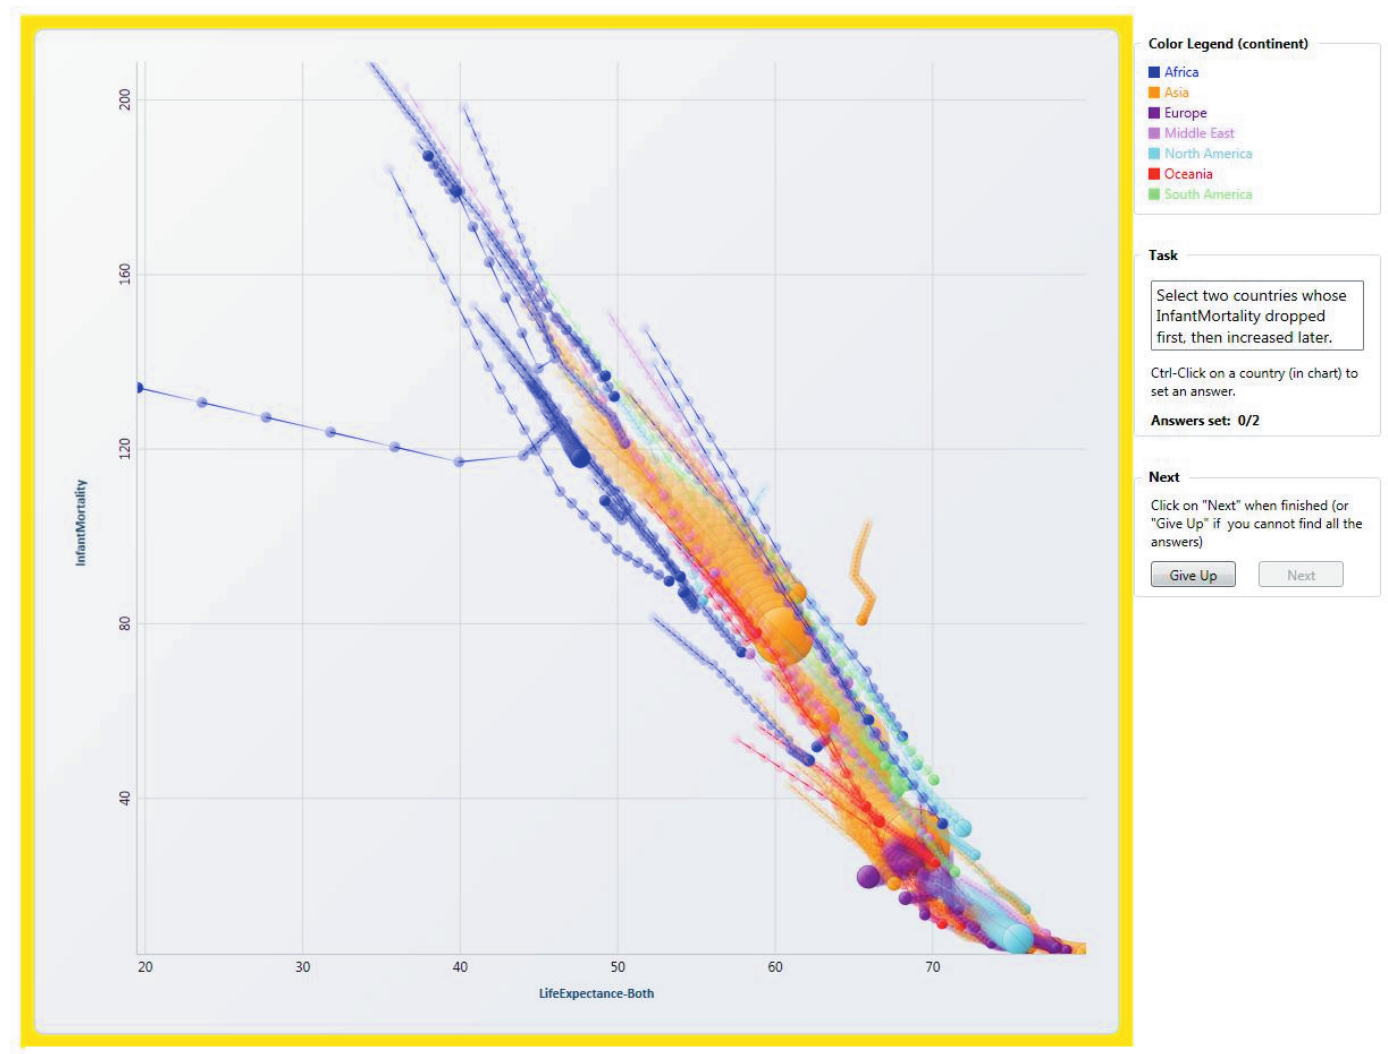
\includegraphics[width=7cm]{./images/Robertson}
\captionof{figure}{\textit{This image shows the trace lines of the graph animation. The traces visualisation shows bubbles at all x and y locations throughout the time frame. This is a conversion of an animation into a static image \cite{Rebortson}.}}
\label{fig:Robertson}
\endgroup


\textbf{Title:} \textit{Design Considerations for Optimizing Storyline Visualizations}
\begin{enumerate}
\item \textit{Definition:} Storyline visualization is a technique that portrays the temporal dynamics of social interactions by projecting the timeline of the interaction onto an axis \cite{Tanahashi}.
\item \textit{The Concept:} Tanahashi and Ma present a storyline visualization which consists of a series of lines, from left to
right along the time-axis, that converge and diverge in the course of their paths \cite{Tanahashi}.
\item \textit{Algorithm:} The algorithm overview is shown in figure \ref{fig:Tanahashi2012}.
\begin{enumerate}
\item Layout of Interaction Sessions: The layout is based on a set of horizontal slots that divide the screen space along the y-axis. Each of these slots has the capacity to accommodate blocks of interaction sessions as long as they do not overlap in time \cite{Tanahashi}.
\item Rearranging Lines: This step takes the slot-based layout of interaction sessions derived from a genome and determines the order of the line segments in each interaction session and its alignment in order to reduce unnecessary wiggles and crossovers \cite{Tanahashi}.
\item Removing White Spaces: In order to prevent such misleading effects, it is critical for the layout computation to include the removal of unnecessary white space to determine the final layout \cite{Tanahashi}.
\end{enumerate}
\item \textit{Related Work:}  This paper is based on the idea of XKCD's hand-drawn illusion "Movie Narrative Charts" \cite{Ogievetsky2009} and develop a algorithm to general storyline visualization.
\item \textit{In this paper, the following visualization techniques are illustrated :} 
\begin{enumerate}
\item Line chart, interactive storyline graph
\item Information visualization/static transitions
\end{enumerate}
\end{enumerate}

\begingroup
\centering
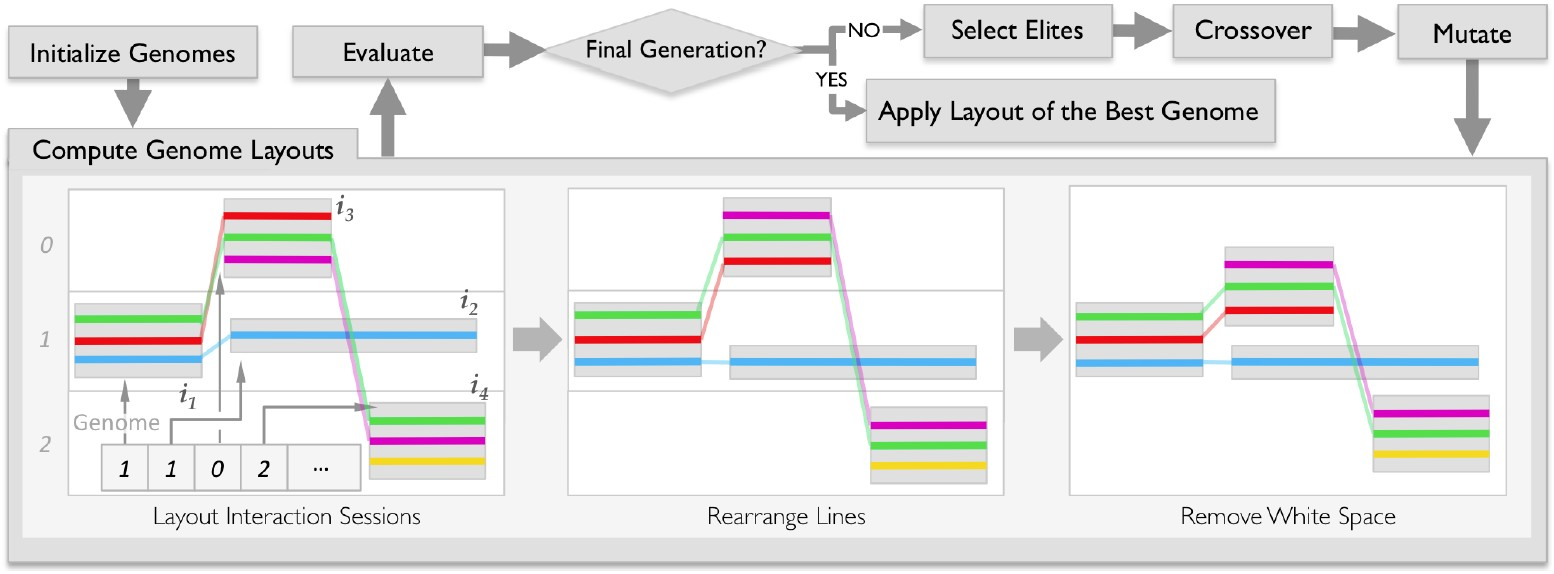
\includegraphics[width=8cm]{./images/Tanahashi2012}
\captionof{figure}{\textit{This shows the overview algorithm of generating storyline visualization \cite{Tanahashi}.}}\label{fig:Tanahashi2012}
\endgroup



\textbf{Title:} \textit{StoryFlow: Tracking the Evolution of Stories}
\begin{enumerate}
\item \textit{Definition:} Storyline visualizations, aim to illustrate the dynamic relationships between entities in a story \cite{shixia}.
\item \textit{The Concept:} Liu et al design a storyline visualization system, StoryFlow, to generate an aesthetically pleasing and legible storyline visualization. It supports real-time user interaction, hierarchical relationships among entities, and the rendering of a large number of entity lines \cite{shixia}.
\item \textit{Theory and application}
\begin{enumerate}
\item StoryFlow: The layout pipeline consists of four steps: relationship tree generation, session/line ordering, session/line alignment, and layout compaction. In the first step, StoryFlow creates a set of dynamic relationship trees for different time frames. Then the relationship trees are used to order sessions and entity lines. Next, sessions/lines between successive time frames are aligned to maximize the number of straight lines in the layout. Finally, a quadratic optimization algorithm is performed to obtain a compact storyline layout, see figure \ref{fig:Liu2013Story} \cite{shixia}.
\end{enumerate}
\item \textit{Related Work:}  This paper is based on previous work of Tanahashi et al \cite{Tanahashi}. Liu et al add support for real-time interaction, hierarchical relationships,and a large number of entity lines. 
\item \textit{In this paper, the following visualization techniques are illustrated :} 
\begin{enumerate}
\item line chart, interactive storyline graph
\item from story to data
\item information visualization/static transitions
\end{enumerate}
\end{enumerate}


\begingroup
\centering
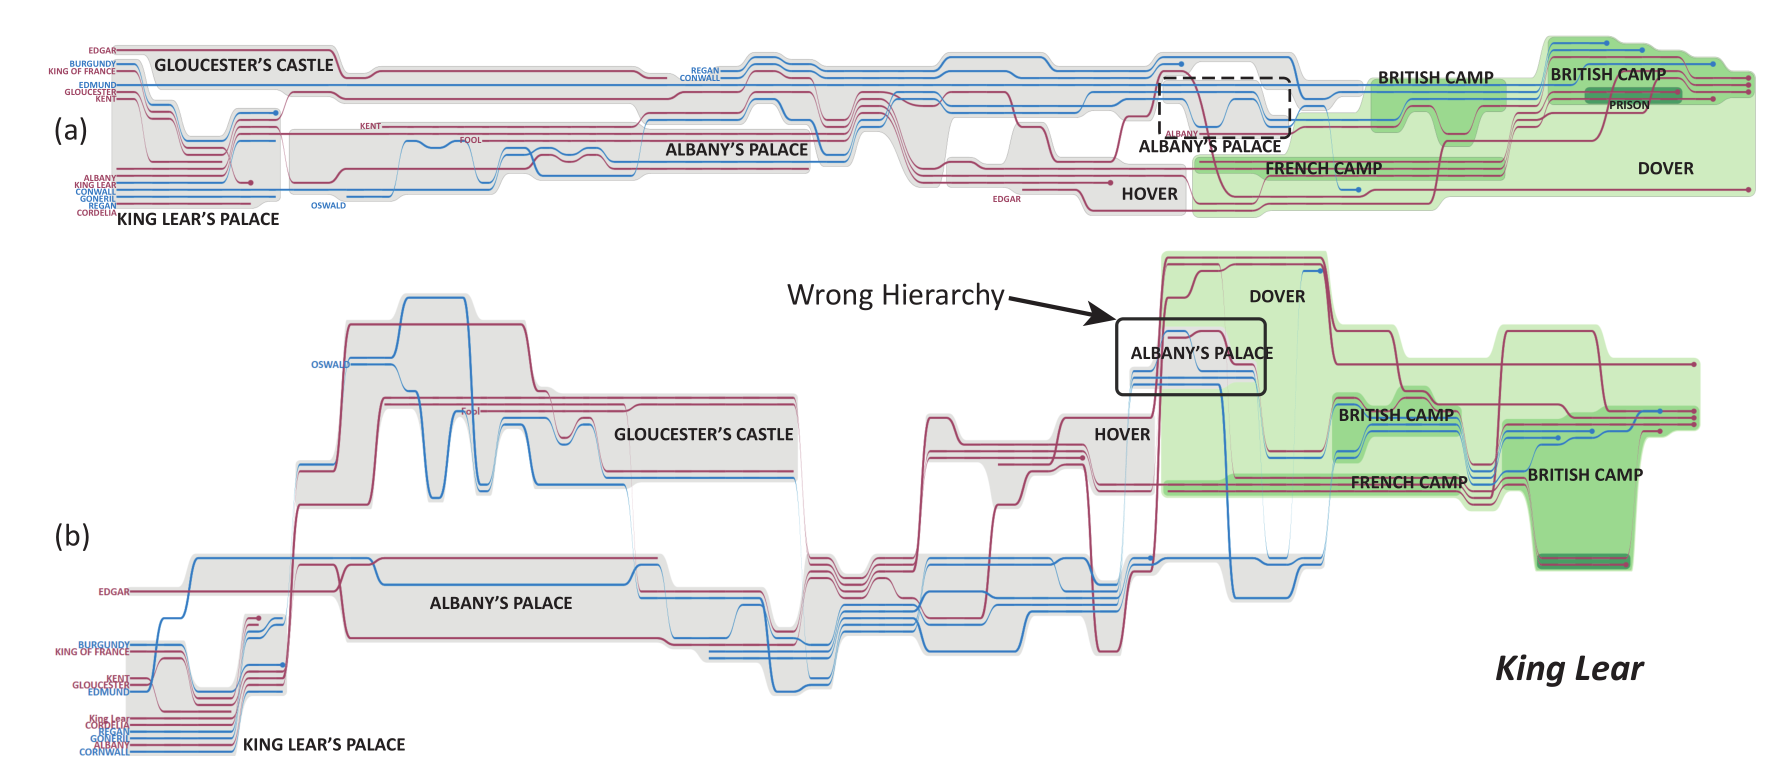
\includegraphics[width=7cm]{./images/Liu2013Story}
\captionof{figure}{\textit{Comparison of King Lear using both methods of layout; (a) - StoryFlow, (b) -  previous method by Tanahashi and Ma \cite{Tanahashi}. The StoryFlow layout presented in this paper focuses on minimising white space and efficiently ordering the story lines to ensure the most concise visual representation of a story. Intersecting lines represent interaction between characters and major events in the story are labeled to add clarity to the visualization \cite{shixia}.}}\label{fig:Liu2013Story}
\endgroup



\subsection{Geo-spatial Visualization}
\textbf{Title:} \textit{Visual Exploration of Big Spatio-Temporal Urban Data: A Study of New York City Taxi Trips} 
\begin{enumerate}
\item \textit{Definition:} 
\item \textit{The Concept:} TaxiVis proposes a method of visualizing a large amount of taxi data consisting of both spatial and temporal dimensions. This approach looks at trends over time as opposed to individual taxi trips, visualizing data from a day in length, up to a year. Seasonal events such as thanksgiving and Christmas can be compared in a like-for-like fashion. See figure \ref{fig:ferreira2013} \cite{ferreira2013}.
\item \textit{TaxiVis Components}:
\begin{enumerate}
\item Time Selection Widget: This allows the user to change the time frame of the visualisation. 
\item Map: This is the canvas for the visualisation.
\item Data Summary: A graph of the raw data with time plotted to the X axis and frequency of taxi trips on the Y axis.
\item Visualization: To reduce clutter, a density heat map is used. This can either be as points on the map or averaging out the data within regions on the map. 
\end{enumerate}
\item \textit{Related Work :}  Taxi data is a popular area of research. Among others, Veloso et al explored patterns and trends in taxi ride data looking at the relationship between pick up and drop off points \cite{veloso2011,Veloso}. Liao et al developed a visual analytics system to error check GPS data streamed from taxis \cite{liao2010}. 
\item \textit{In this paper, the following visualization techniques are illustrated :} 
\begin{enumerate}
\item Level of detail visualization, Density Heat maps
\item Geo-spatial visualization/static transitions
\end{enumerate}
\end{enumerate}
\begingroup
\centering
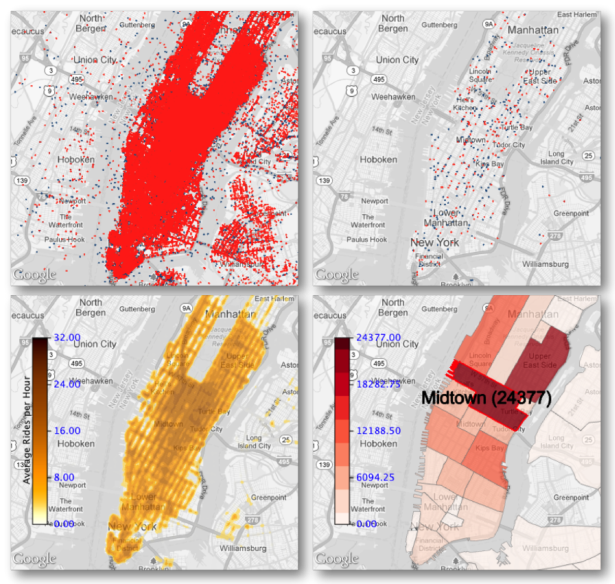
\includegraphics[width=7cm]{./images/ferreira2013}
\captionof{figure}{\textit{The top left image shows the trips rendered on the map. However the cluttered view can be reduced by employing a level-of-detail approach (top right) which takes a subsample based off the order in which the trips occurred. The bottom left image shows a density heat map of the taxi trips whereas the bottom right image averages out the data in each region to make a regional density heat map \cite{ferreira2013}.}}\label{fig:ferreira2013}
\endgroup

\section{Animated Transition}
\textbf{Title:} \textit{Does Animation in User Interfaces Improve Decision Making}
\begin{enumerate}
\item \textit{Definition:} Gonzalez and Cleotilde define animation as a series of varying images presented dynamically according to user actions in ways that help the user to perceive a continuous change over time and develop a more appropriate mental model of the task \cite{gonzalez1995animation}.
\item \textit{The Concept:} The results of this study show that decision making performance is highly contingent on the properties of the animation user interface such as image realism, transition smoothness, and interactivity style, and also sensitive to the task domain and the user's experience.  
\item \textit{Case study:}
\begin{enumerate}
\item values of accuracy, time, ease of use, and enjoyability for the two types of images, transitions, and interactivity styles indicated that realistic images, gradual transitions, and parallel interactivity produced better decision.
\item decision making accuracy, time, ease of use, and enjoyability in animated interfaces are influenced by the form of image representation, the transition effects, and the form of interactivity.
\item This research supports the idea that to be an effective decision support tool, animation must be smooth, simple, interactive and explicitly account for the appropriateness of the user's mental model of the task.
\end{enumerate}
\item \textit{Related Work:} This paper reviews selected empirical investigations from the literature in Education, Psychology, and HCI which suggest that animation may make interfaces easier, more enjoyable, and understandable and study the effect of animation on decision making \cite{gonzalez1996does}.
\end{enumerate}


\subsection{Scientific Visualization}
\textbf{Title:} \textit{AniVis:A Template-Based Animation Tool for Volume Visualization}
\begin{enumerate}
\item \textit{Definition:} 
\item \textit{The Concept:} This paper introduces animation tool named: AniVis for scientific visualization exploration and communication. This tool can turn the results of data exploration and visualization into animation content and the users can create a complex animation sequence by combining several simple effects \cite{Akiba}.
\item \textit{Tools operator:}
\begin{enumerate}
\item Parameter-space blending: This operator creates intermediate frames between two instances of frames I1 and I2 by interpolating their respective parameters. If I1 and I2 do not overlap in time, they generate intermediate frames by interpolating the parameters of the last frame of I1 and the first frame of I2. Otherwise, they generate intermediate frames by interpolating the parameters of their corresponding frames \cite{Akiba}.

\item Image-space blending: This operator creates the animation content between I1 and I2 by interpolating their respective image frames. Similarly to parameter-space blending, if I1 and I2 don't overlap in time, they generate intermediate frames by blending the last frame of I1 and the first frame of I2. The effect is that the last frame of I1 gradually fades out as the first frame of I2 gradually fades in. If I1 and I2 overlap, they generate intermediate frames by blending \cite{Akiba}.

\item Playback. This operator lets users repeatedly loop through one or more consecutive instances of interest \cite{Akiba}.

\end{enumerate}

\item \textit{Case study}
\begin{enumerate}
\item MRI Head Data: This case study focuses on highlighting a brain tumor. The animation comprised of four pieces of animation content. The first is a spatial overview that rotates the volume data 360 degrees along the y-axis. The second piece is a spatial exploration in which the user customizes the view. The third is a parameter-space blending between a spatial exploration and a slicing, which reveals a tumor's inner structure.  The last piece is a parameter-space blending between a spatial exploration and highlighting, which highlights a tumor by varying the opacity while zooming in on the region of interest. See figure \ref{fig:AniVis} \cite{Akiba}.
\item Hurricane Data: This case study  has five components. The first is a caption showing the animation's content, blended with a spatial exploration that zooms in on the data. The second piece is a temporal exploration to show early time steps. The third is a variable overview that browses through three data attributes: vapor, wind speed, and cloud. The fourth piece is a temporal exploration to show later time steps. The fifth is a spatial exploration that zooms in on the hurricane's eye \cite{Akiba}.
\end{enumerate}
\item \textit{Related Work:}  This paper is based on previous animation support \cite{childs} and an animation enhanced system \cite{correa} and develops a template-based visualization tools for animation. 
\item \textit{In this paper, the following visualization techniques are illustrated :} 
\begin{enumerate}
\item illustrative volume rendering, static and animated graphs, slicing
\item scientific visualization, transitions
\end{enumerate}
\end{enumerate}


\begingroup
\centering
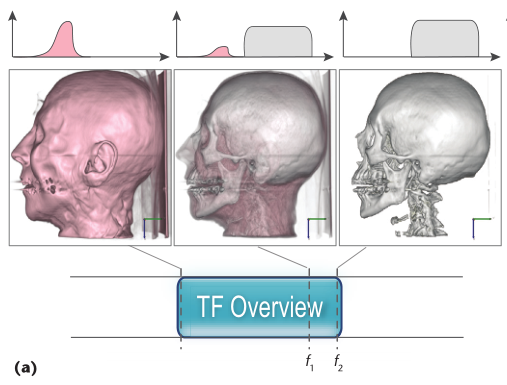
\includegraphics[width=8cm]{./images/AniVis}
\captionof{figure}{\textit{This image shows the AniVis animation tool displaying MRI scan data. By blending the two layers of data together, a new layer of information is revealed (middle image) \cite{Akiba}.}}\label{fig:AniVis}
\endgroup


\subsection{Information Visualization}
\textbf{Title:} \textit{Does Animation Help Users Build Mental Maps of Spatial Information?}
\begin{enumerate}
\item \textit{Definition:} 
\item \textit{The Concept:} This paper examines how animating a viewpoint change in a spatial information system affects a user's ability to build a mental map of the information in the space. Based on a user-study involving a spatial map of a family tree, animation improved subjects' ability to learn the spatial position of family members within the tree without a speed penalty \cite{bedrson}.
\item \textit{Experiment:} Family Tree test: two different family trees of nine individuals are presented to two groups people with animation and without animation. The subjects were given three kinds of tasks : navigation of family trees, exploratory family trees and reconstruction of family trees, and the accuracy of performance are recorded. In this experiment, there is a statistically significant improvement in accuracy of the reconstruction task than other tasks. Animation resulted in fewer task errors than the static ones. See figure \ref{fig:bederson99does}.
\item \textit{Related Work:} This paper based on Gonzalez \cite{gonzalez} and Donskoy \cite{donskoy} which is about the relationship between animation and users' understanding. Compared to previous work, this paper focuses on animation of the viewpoint. The performance of experiment is change from single in-between frame to several in-between frames.
\item \textit{In this paper, the following visualization techniques are illustrated :} 
\begin{enumerate}
\item hierarchical graph, animated graphs
\item static graphs
\item information visualization/ animated transitions
\end{enumerate}
\end{enumerate}


\begingroup
\centering
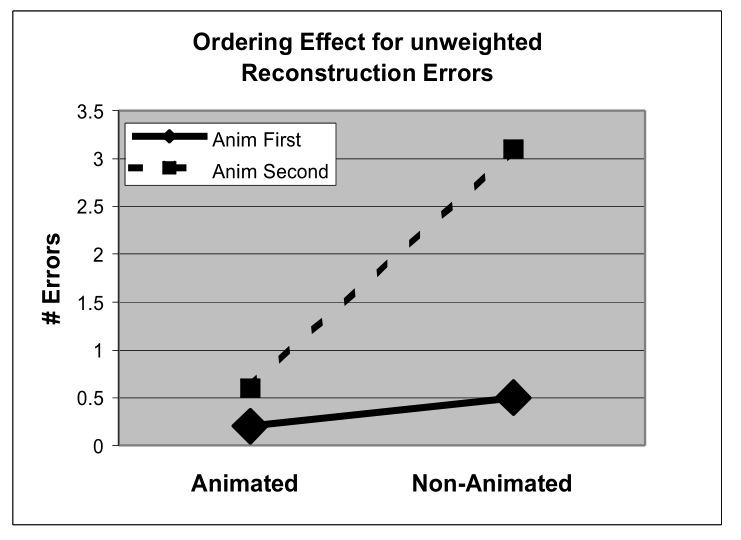
\includegraphics[width=7cm]{./images/bederson99does}
\captionof{figure}{\textit{This shows the ordering effects when presenting an animated and non-animated graphic. If the animated graphic is shown first then there is little difference in recall error, however, if the animation graphic is shown second then the recall error is significantly higher for the non-animated graphic \cite{bedrson}.}}
\label{fig:bederson99does}
\endgroup



\textbf{Title:} \textit{Animated Transitions in Statistical Data Graphics}
\begin{enumerate}
\item \textit{Definition:} 
\item \textit{The Concept:} This paper investigates the effectiveness of animated transitions in traditional statistical data graphs, such as bar charts, pie charts, and scatter plots. A visualisation framework called DynaVis was created to test the effectiveness of animation on the user's preference and information retention. Graph animations are used to keep viewers engaged and to promote creative thinking about the data. See figure \ref{fig:Heer2007} \cite{heer2007}.
\item  \textit{DynaVis:} 
\begin{enumerate}
\item The software displays animated transitions of statistical data graphs. Sorting and filtering animation provide the user insight into the composition of the data. All transitions take place over a time frame rather than instantaneously so the user can see exactly how the visualisation has changed. Animations between different graph types are implemented by morphing the data from one shape and size to another.
\item Statistically significant differences in user preference were found between static graphs and animated graphs. Animated transitions can improve graphical perception. This was reflected in the findings of the user experiments testing recall and understanding. However, not all transition scenarios were found to be significantly different.
\end{enumerate}
\item \textit{Related Work:}  This paper was based off the previous work of Bederson and Boltman \cite{bedrson} but builds upon it by testing different transitional events.
\item \textit{In this paper, the following visualization techniques are illustrated :} 
\begin{enumerate}
\item pie charts, bar charts, scatter plot, animation
\item information visualization/animated transitions
\end{enumerate}
\end{enumerate}

\begingroup
\centering
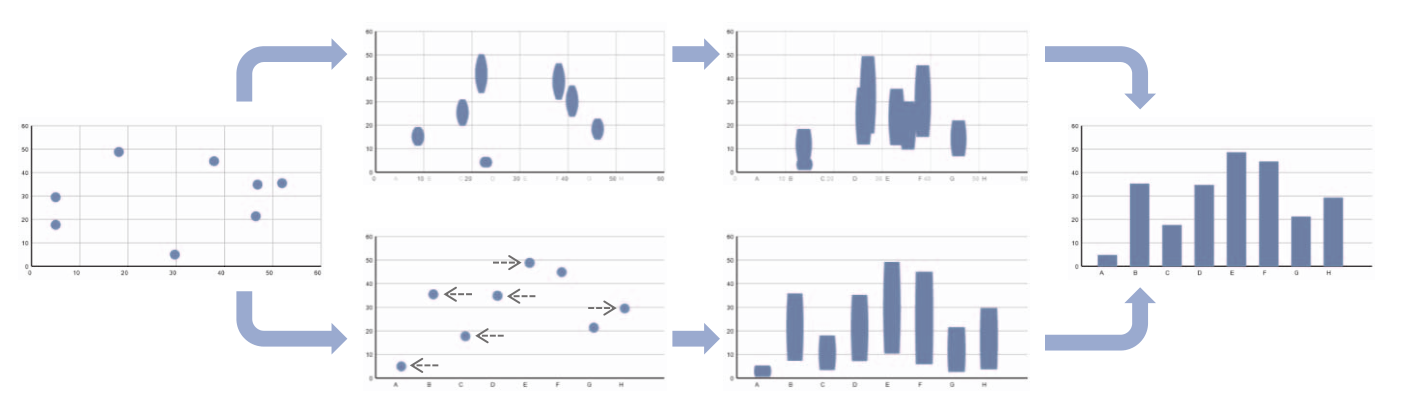
\includegraphics[width=8cm]{./images/AnimatedTransitions}
\captionof{figure}{\textit{This figure shows the process of transition for a scatter plot to a bar chart. The top path starts by stretching the points to size and then moving to the right location, whereas the bottom path moves the dots first, then resizes and reshapes them \cite{heer2007}. }}
\label{fig:Heer2007}
\endgroup



\section{Memorability}
Memory refers to the faculty by which things are remembered; the capacity for retaining, perpetuating, or reviving the thought of things past according to The Oxford English Dictionary \cite{memory}. Memorability is an important goal of storytelling. A good visualization technique will draw the viewer's attention and increase a story's memorability \cite{bateman}.

\textbf{Title:} \textit{What Makes a Visualization Memorable?}
\begin{enumerate}
\item \textit{Definition:} 
\item \textit{The Concept:} Borkin et al\cite{borkin2013makes} develop an online memorability study over 2000 static visualizations that cover the large variety of visualizations and determine which visualization types and attributes are more memorable. They investigate a domain at the interface between human cognition and visualization design.
\item \textit{Case Study:} 
\begin{enumerate}
\item Visualization taxonomy: The taxonomy classifies static visualizations according to the underlying data structures, the visual encoding of the data, and the perceptual tasks enabled by these encodings. It features twelve main visualization categories and several popular sub-types for each category.
\item Memorability experiment: Borkin et al run memorability test via Amazon's Mechanical Turk with 261 participants and gather memorability scores.
\item Experiment result: The result in memorability comparison test demonstrates that there is memorability consistency with scenes, faces, and also visualizations, thus memorability is a generic principle with possibly similar generic, abstract, features. And the result in visualization attribute test illustrates that higher memorability scores were correlated with visualizations containing pictograms, more color, low data-to-ink ratios, and high visual densities.
\item Conclusion: Borkin et al. show that visualizations are intrinsically memorable with consistency across people. Visualizations with low data-to-ink ratios and high visual densities (i.e., more chart junk and "clutter") were more memorable than minimal, "clean" visualizations \cite{borkin2013makes}. 

\end{enumerate}
\end{enumerate}


All papers in this section evaluate the effects of visualization on memorability. Bateman et al \cite{bateman} explore the effects of embellishment on comprehension and memorability. And Saket et al \cite{saket2015} illustrate that map-based visualization can improve accuracy of recall data comparing with node-link visualization.


\subsection{Storytelling In Information Visualization And Memorability}
\textbf{Title:} \textit{Useful Junk? The Effects of Visual Embellishment on Comprehension and Memorability of Charts}
\begin{enumerate}
\item \textit{Definition:} 
\item \textit{The Concept:} This paper examines whether embellishment is useful for comprehension and memorability of charts. Bateman et al compare plain and embellished charts, and conclude that a user's accuracy in describing the embellished charts is no worse than for plain charts, and that their recall after a two-to-three week gap is significantly better \cite{bateman}. 
\item \textit{Experiment:} A comparison of plain and embellished charts: 14 embellished charts are selected from Nigel Holmes' book Designer's Guide to Creating 
Charts and Diagrams \cite{holmes}, and converted to plain charts. See figure \ref{fig:Bateman2010Effects}. Twenty participants are presented a chart on a slide, alternating between embellished and plain versions. Participants are required to perform two tasks (reading and describing task and recall task) after five-minutes and after 2-3 weeks. The eye-gaze and task performance of participants are recorded for analysis. This study shows that there is no significant difference between plain and embellished version for interactive interpretation accuracy and recall accuracy after a five-minute gap,
but after a long-term gap, recall of both topic and detail of chart(categories and trend) is significant better for embellishment charts. Participants saw the value in message more often in Holmes charts than in the plain charts.

\item \textit{Related Work:}  Previous studies have suggested that minor decoration in charts may not hamper interpretation \cite{Blasio}, and work in psychology has shown that the use of imagery can affect memorability \cite{gambrell}, but there is very little work that looks at how chart imagery can affect the way people view information charts. 
\item \textit{In this paper, the following visualization techniques are illustrated :} 
\begin{enumerate}
\item bar charts, line charts, embellished charts, pie charts, static graph
\item Information visualization/memorability
\end{enumerate}
\end{enumerate}

\begingroup
\centering
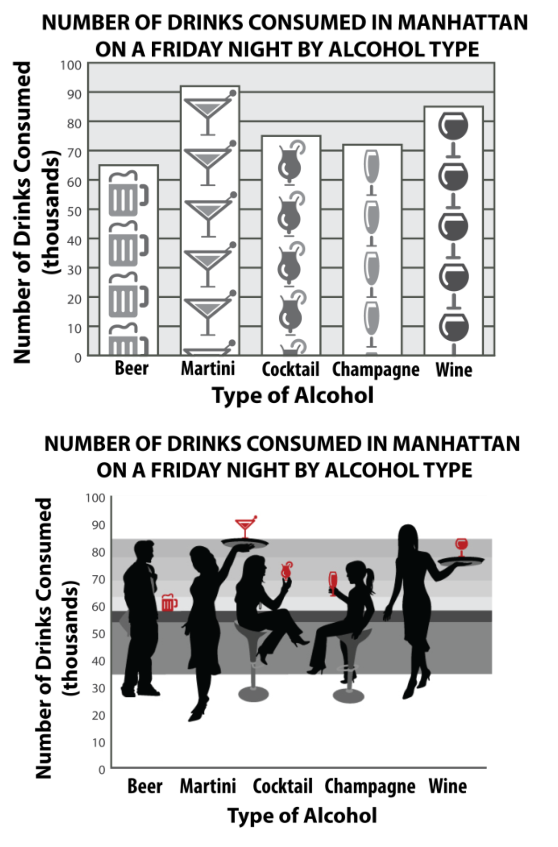
\includegraphics[width=7cm]{./images/Bateman2010Effects}
\captionof{figure}{\textit{This graphic compares two different levels of graphical embellishment of the same data. The top graph is an embellished image but still retains the recognisable features of a bar chart. The bottom image replaces the bars with a silhouette of a person next to a drink where the height of the drink corresponds to the height of the original bar. This method also uses the addition of colour to emphasise the data \cite{bateman}.}}\label{fig:Bateman2010Effects}
\endgroup

\subsection{Storytelling In Geo-spatial Visualization And Memorability}
\textbf{Title:} \textit{Map-based Visualizations Increase Recall Accuracy of Data}
\begin{enumerate}
\item \textit{Definition:}  
\item \textit{The Concept:} Saket et al. illustrate that different visualization designs can effect the recall accuracy of data visualized. Comparing with node-link visualization, map-based visualization is more effective \cite{saket2015}.
\item  \textit{Experiment:} 
\begin{enumerate}
\item Two dataset are examined. A book dataset (small) and LastFM dataset (large), are transformed into a node-link visualization and node-link group visualization (map-based). See Figure \ref{fig:saket2015}.
\item Three phrases are performed to examine the difference between node-link visualization and map-based visualization. In phase 1 participants examine two kinds of visualization without task with unlimited time. Phase 2 ask participant to study two kinds of visualization with six tasks in required time. Phase 3 ask participants to recall what they read in phase 1 and 2, complete 6 tasks similar to phase 2,and 3 new addition task \cite{saket2015}.
\item The result of experiment illustrates that recalling map-based diagrams is more accurate than recalling node-link diagrams, but no faster.
The participants spent more time on map-based visualizations than node-link visualizations \cite{saket2015}.  
\end{enumerate}
\item \textit{Related Work:} This paper is based on previous work of visualization memorability \cite{bateman} and a recalling experiment \cite{isola2011}
\item \textit{In this paper, the following visualization techniques are illustrated :} 
\begin{enumerate}
\item geographic information visualization, node-link diagram, map-based diagram
\item Geo-spatial visualization/Memorability
\end{enumerate}
\end{enumerate}
\begingroup
\centering
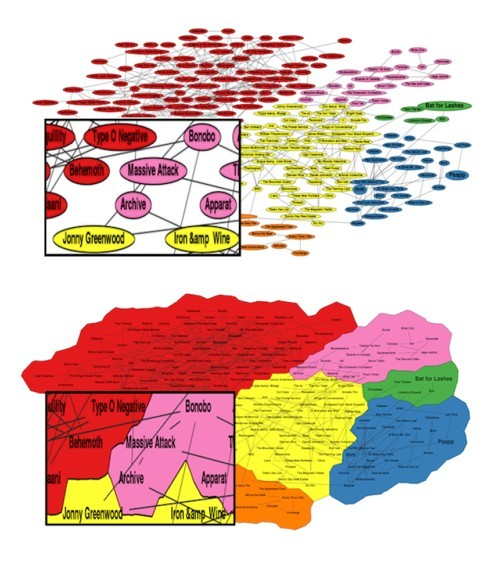
\includegraphics[width=6cm]{./images/saket2015}
\captionof{figure}{\textit{This figure shows two visualization of the same data: node-link diagram and map-based diagram \cite{saket2015}.}}
\label{fig:saket2015}
\endgroup




\section{interpretation}
\subsection{Scientific Visualization}
\textbf{Title:} \textit{Scientific Storytelling using Visualization}
\begin{enumerate}
\item \textit{Definition:} Ma et al \cite{sci} state that a story that is well paced exhibits deliberate control over the rate at which plot points occur.
\item \textit{The Concept:} This paper presents a selection of scientific storytelling visualization from NASA related work and describes various examples.
\item  \textit{Examples and Applications :} 
\begin{enumerate}
\item Visualization at a Scientific Research Center: The Scientific Visualization Studio (SVS) at NASA uses storytelling visualization to investigate observational data collected by instruments and sensors and make it more suitable for consumption by the public \cite{nasa}\cite{svs1}.
\item Visualization at a Science Museum: The science museum presents visualization to the public with complex and abstract geographic phenomena at extreme size scales for explanatory animations. The science museums provide more interpretation through labels, videos, and live demonstrations. See figure \ref{fig:Scientific_Storytelling_CGA}\cite{sci}.
\item Storytelling using interactive Visualization: Storytelling enables the user to interact with geographic data such as the Earth's climate or the collapse of a star by using a story model, such as story nodes or story transitions\cite{Akiba}.
\end{enumerate}
\item \textit{Related Work :} This paper is based on previous scientific visualization work at U.S. NASA, based in scientific research centre and scientific museum and describe how  visualization can be used to tell a good story, and tell it well. This is a topic that the scientific visualization research community paid little attention to at that time.
\item \textit{In this paper, the following visualization techniques are illustrated :} 
\begin{enumerate}
\item 3D Stereoscopic displays, story boards, Hyper-wall, touch display, geographic information visualization, animation
\item from data to story
\item Geo-spatial visualization/interpretation
\end{enumerate}
\end{enumerate}

\begingroup
\centering
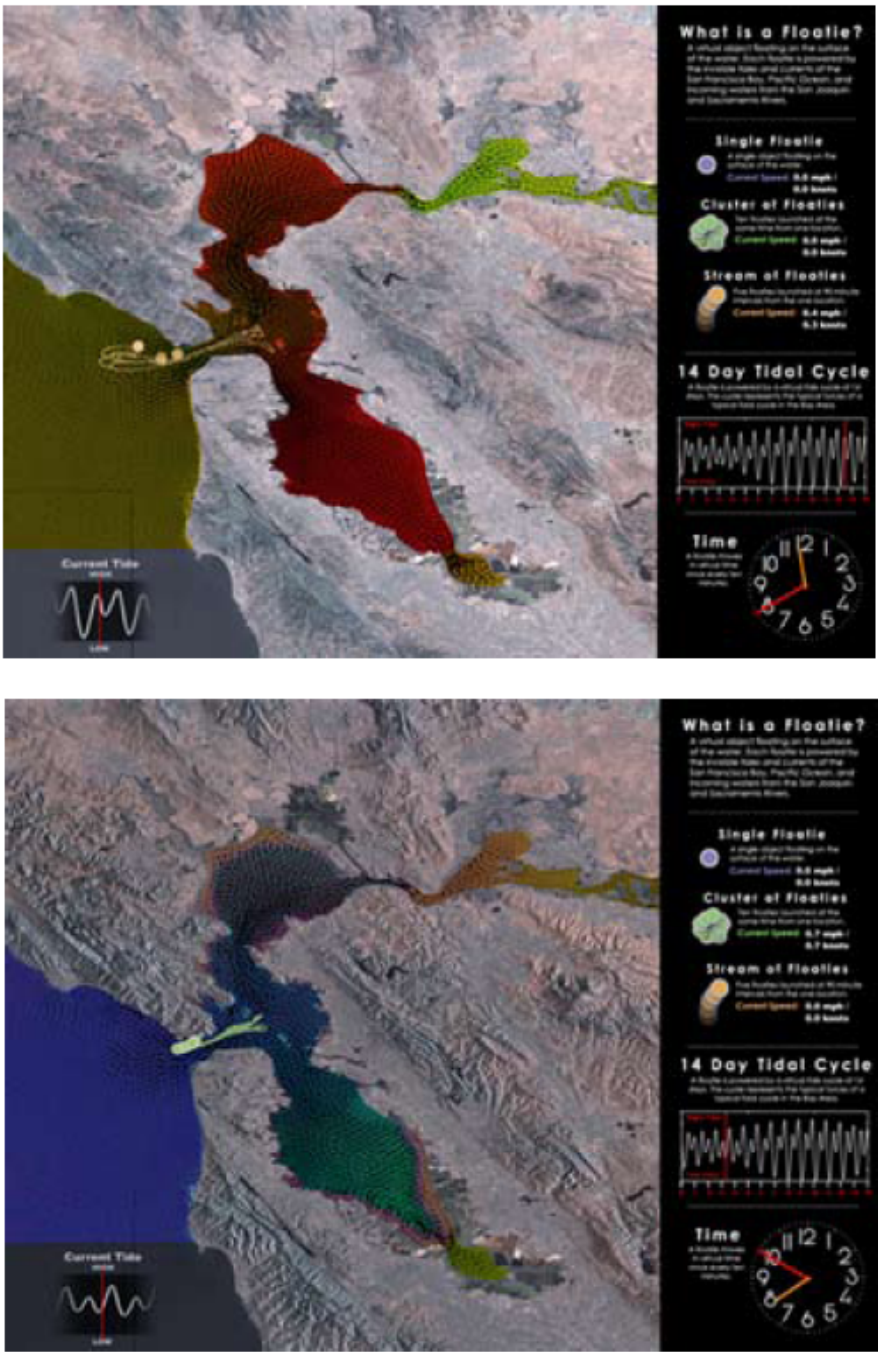
\includegraphics[width=8cm]{./images/Scientific_Storytelling_CGA}
\captionof{figure}{\textit{The interactive software used at the Exploratorium in San Francisco. The purpose of this software is to educate users on the process of how tides, currents and rivers combine in the estuary of San Francisco bay. A touch-screen is used to place floats into the virtual water so that the user can see the effects of the current on the float. Users can watch the effects of predicted tide and river flow cycles on the floats trajectory. Other contextual information is provided as an animation alongside the visualization \cite{sci}.}}
\label{fig:Scientific_Storytelling_CGA}
\endgroup


\subsection{Information Visualization}
\textbf{Title:} \textit{Storytelling: The Next Step For Visualization}
\begin{enumerate}
\item \textit{Definition:} Kosara and Mackinlay define a story as an ordered sequence of steps, with a clearly defined path through it \cite{Kosara}.
\item \textit{The Concept:} This paper presents a selection of previous work on storytelling in visualization and postulates storytelling as a fruitful area of future research \cite{Kosara}.
\item  \textit{Examples and Applications:} 
\begin{enumerate}
\item Gapminder, Human Development Index: The Gapminder visualization uses animated bubble charts to show possible detrimental effects on a person's ability to follow trends \cite{Rebortson}. A continent is mapped to color, region is mapped to each bubble, population is mapped to bubble size, position is mapped to average yearly income.
\item New York Times, Copenhagen: \textit{The New York Times} visualization illustrates how interaction provides a way of navigating through events by using line charts, which should be supported by a well-constructed story. Color represents different countries and the x-axis represents time and the y-axis represents a standard of industry index.
\item Minard's map of Napoleon's Russian Campaign : The storytelling visualization in this example presents a range of data attributes.  The size of army, the path of march and temperature are shown in same graph. The width of the line represents the number of men in the army, the x-axis represents the time and the y-axis represents location and temperature. See Figure \ref{fig:StorytellingTheNextStepForVisualisation}.
\end{enumerate}
\item \textit{Related Work :} This paper is based on  the previous history of storytelling, definition and model of Segel and Heer research \cite{segal} and outlines a research program to develop storytelling as a visualization task of equal importance to exploration and analysis. Previous visualization is focused on novel techniques. This gave rise to evaluation papers 
that compared techniques, and tried to ascertain the perceptual mechanisms behind specific techniques.
\item \textit{In this paper, the following visualization techniques are illustrated :} 
\begin{enumerate}
\item stacked area charts, bubble charts, line charts, animation
\item information visualization/interpretation
\end{enumerate}
\end{enumerate}


\begingroup
\centering
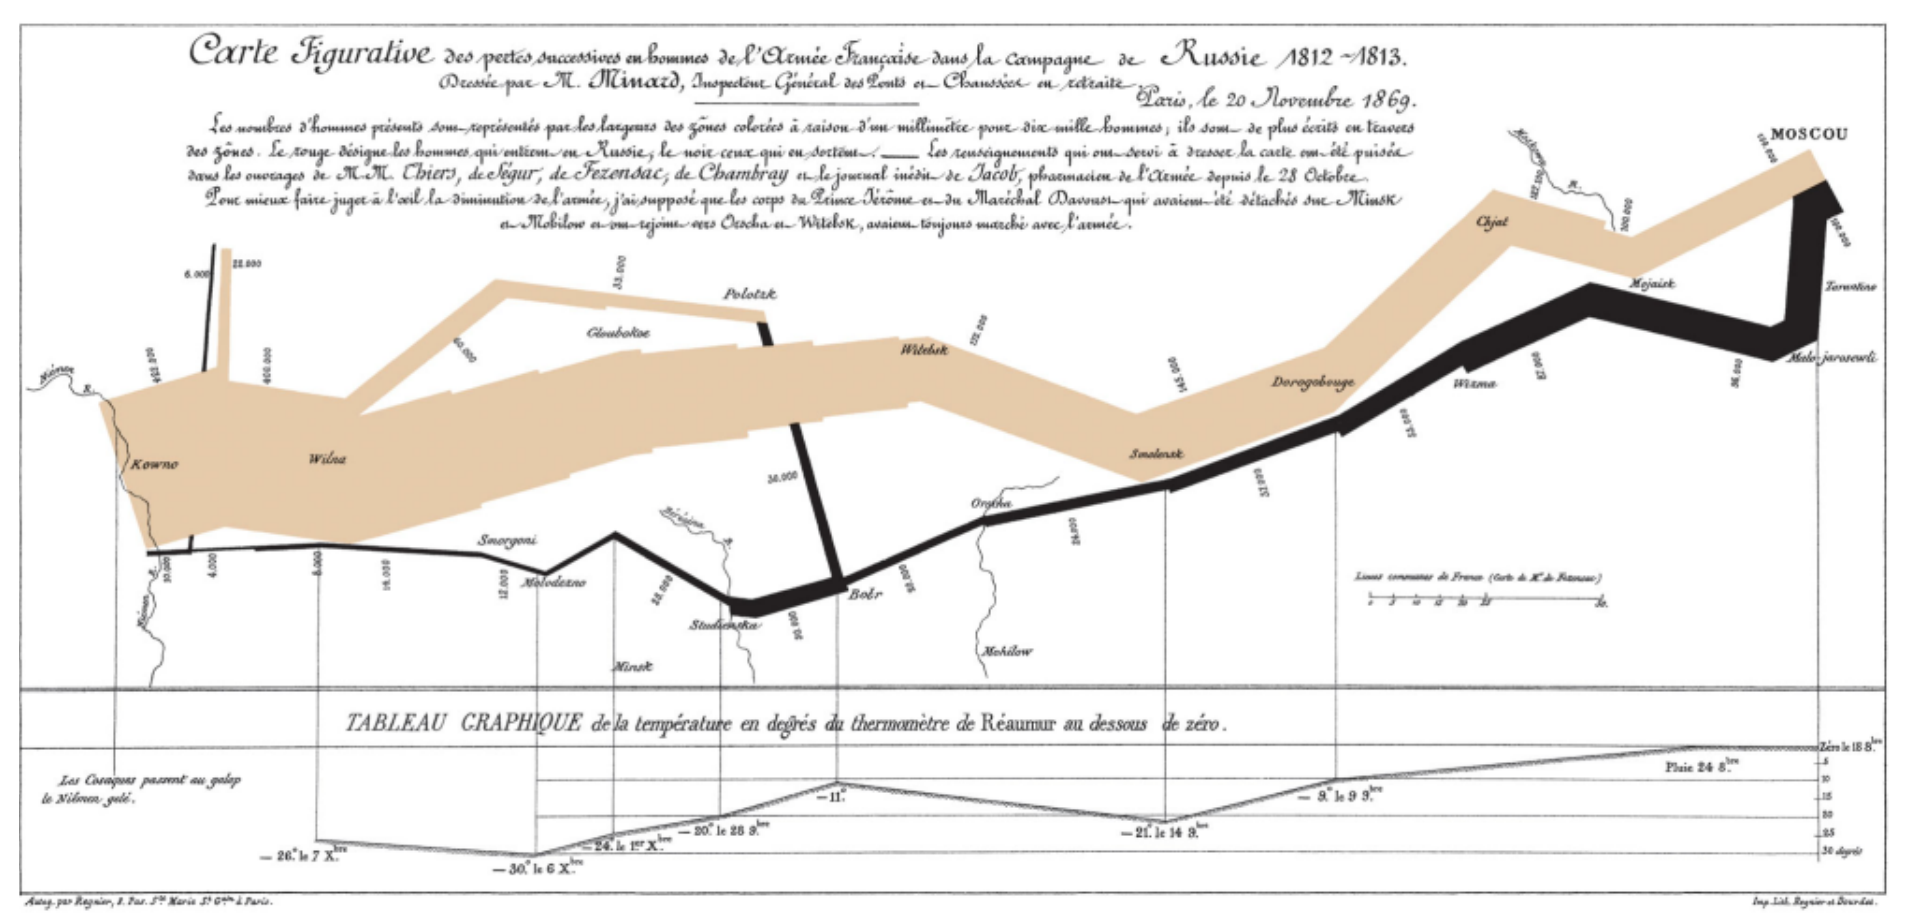
\includegraphics[width=7cm]{./images/StorytellingTheNextStepForVisualisation}
\captionof{figure}{\textit{Here is Minard's famous illustration of fatalities caused during Napoleon's attach on Moscow. It depicts the size of the army throughout the campaign, thinning at each battle. Although descriptive, the flow of data only loosely corresponds to time due to the tangents the line take. In addition to the army size line, the temperature is also referenced at the bottom so death rates can be directly compared \cite{Kosara}.}}
\label{fig:StorytellingTheNextStepForVisualisation}
\endgroup


\section{summary}
This survey provides a novel up-to-date overview of storytelling in visualization. The most important recent literature is included and discussed. Since storytelling in visualization is a recently new subject, we expect an increase over the next few years. Moreover we believe it will evolve into popular topic in visualization.


According to Table \ref{table:classification1}, the storytelling visualization focuses on information visualization more than scientific visualization, which conveys that ore problems are left unsolved. However, by developing a storytelling model in Scientific visualization \cite{wohlfart2}, the implementation of storytelling in scientific visualization could increase in the future. On the other hand, storytelling in visualization concentrates more on exploration than on presentation. Like  Kosara and Mackinlay \cite{Kosara} state that visualization techniques address the exploration and analysis of data more than presenting data.

In future work, there are many directions and unsolved problems, such as scientific visualization storytelling for presentation, dynamic storytelling in scientific visualization. And storytelling will gain importance in data presentation and data exploration.



\newpage
%\bibliographystyle{eg-alpha}
\bibliographystyle{eg-alpha-doi}

\bibliography{egbibsample}

\end{document}

